%% LyX 2.3.1 created this file.  For more info, see http://www.lyx.org/.
%% Do not edit unless you really know what you are doing.
\documentclass[12pt,english,letterpaper]{kuthesis}
\usepackage{mathptmx}
\renewcommand{\sfdefault}{lmss}
\renewcommand{\ttdefault}{lmtt}
\usepackage[T1]{fontenc}
\usepackage[utf8]{inputenc}
\usepackage{geometry}
\geometry{verbose,tmargin=1in,bmargin=1in,lmargin=1in,rmargin=1in}
\setcounter{secnumdepth}{3}
\setcounter{tocdepth}{3}
\usepackage{color}
\usepackage{babel}
\usepackage{amsmath,amsfonts,amssymb,mathtools}
\usepackage{bm}
\usepackage{algorithm} %
\usepackage[noend]{algpseudocode} %
\usepackage{url}
\usepackage{graphicx}
\usepackage{tikz}
\usepackage{setspace}
\usepackage{esint}
\usepackage[authoryear]{natbib}
\doublespacing
\usepackage[unicode=true,
 bookmarks=true,bookmarksnumbered=false,bookmarksopen=false,
 breaklinks=true,pdfborder={0 0 0},pdfborderstyle={},backref=false,colorlinks=true]
 {hyperref}
\hypersetup{pdftitle={University of Kansas Thesis Template},
 pdfauthor={Anonymous},
 pdfsubject={A Thesis},
 urlcolor={black},citecolor={black},allcolors={black}}

\makeatletter

%%%%%%%%%%%%%%%%%%%%%%%%%%%%%% TiKz
%\input{stylefiles/setupSEMstyle}
%\tikzstyle{o}=[shape=circle,fill=yellow!60!orange!90,draw=black!80,thick,minimum width=1.1cm]

%%%%%%%%%%%%%%%%%%%%%%%%%%%%%% LyX specific LaTeX commands.
\providecommand{\LyX}{\texorpdfstring%
  {L\kern-.1667em\lower.25em\hbox{Y}\kern-.125emX\@}
  {LyX}}
%% Because html converters don't know tabularnewline
\providecommand{\tabularnewline}{\\}

%%%%%%%%%%%%%%%%%%%%%%%%%%%%%% User specified LaTeX commands.
\DeclareMathOperator*{\argmax}{arg\,max}
\DeclareMathOperator*{\argmin}{arg\,min}
\DeclareMathOperator{\tr}{tr}
\DeclareMathOperator{\lb}{\Bigg\{}
\DeclareMathOperator{\rb}{\Bigg\}}
\newcommand{\back}{\texttt{\textbackslash}}
\newcommand{\norm}[1]{\left\lVert{#1}\right\rVert}
\newcommand{\summ}[2]{\mathop{\sum_{#1}}_{#2}}
\newcommand{\matr}[1]{\mathbf{#1}}
\newcommand{\hatmat}[1]{\hat{\mathbf{#1}}}
\newcommand{\hatbm}[1]{\hat{\bm{#1}}}
\newcommand*{\tran}{^{\mkern-1.5mu\mathsf{T}}}
\newcommand{\code}[1]{\texttt{#1}}
\newcommand*{\R}{\mathbb{R}}
\newcommand*{\Ev}[1]{\mathbb{E}\lbrack{#1}\rbrack}
\renewcommand{\L}{\mathcal{L}}
\newcommand*{\E}{\mathcal{E}}
\renewcommand*{\G}{\mathcal{G}}
\newcommand*{\N}{\mathcal{N}}
\newcommand*{\by}{\matr{y}}
\newcommand*{\bY}{\matr{Y}}
\newcommand*{\bmy}{\bar{\matr{y}}}
\newcommand*{\bmY}{\bar{\matr{Y}}}
\newcommand*{\bX}{\matr{X}}
\newcommand*{\bx}{\matr{x}}
\newcommand*{\bmx}{\bar{\matr{x}}}
\newcommand*{\bmX}{\bar{\matr{X}}}
\newcommand*{\I}{\matr{I}}
\newcommand*{\Beta}{\matr{B}}
\newcommand*{\Kappa}{\matr{K}}
\newcommand*{\Rho}{\matr{P}}
\newcommand*{\bOmega}{\bm{\Omega}}
\newcommand*{\bTheta}{\bm{\Theta}}
\newcommand*{\bSigma}{\bm{\Sigma}}
\newcommand*{\bDelta}{\bm{\Delta}}
\newcommand*{\bGamma}{\bm{\Gamma}}
\newcommand*{\bPi}{\bm{\Pi}}
\newcommand*{\bbeta}{\bm{\beta}}
\newcommand*{\eps}{\varepsilon}
\newcommand*{\beps}{\bm{\varepsilon}}
\newcommand*{\bmu}{\bm{\mu}}
\newcommand*{\Var}{\text{Var}}
\newcommand*{\cov}{\text{cov}}
\newcommand*{\Cov}{\text{Cov}}
\renewcommand*{\vec}[1]{\text{vec}({#1})}
\newcommand*{\sign}[1]{\text{sign}({#1})}
\newcommand*{\pinv}[1]{({#1})^{-1}}
\newcommand*{\inv}{^{-1}}
\newcommand*{\hatinv}[1]{\hat{#1}^{-1}}
\newcommand*{\set}[1]{\{{#1}\}}
\newcommand*{\xiny}[2]{{#1}\in\{1,2,\ldots,{#2}\}}
\newcommand*{\diag}[1]{\text{diag}(#1)}

%used to align decimals in tables according to APA style
\usepackage{dcolumn}
\usepackage{booktabs}

% Set the title and author info
\title{Modeling Moderators in Psychological Networks}
\author{Trevor James Swanson}

% Following is OPTIONAL list of previous degrees earned. 
% If there are more than 5 or so, then title pagelayout may become too crowded,
% depending on the number of committee members. 
\priorcreds{B.A. Psychology, Texas Christian University, 2014}{M.A. Psychology, University of Kansas 2014}
% It is acceptable to delete \priorcreds if it is not desired on title page


\dept{Department of Psychology}
\degreetitle{Doctor of Philosophy}
\papertype{Dissertation} %or Thesis (Choose whatever word you want to put on p.2)

%% Committee member names are required for the title page. We make space
%% for as many as 7 members, with various roles/titles.
%% It is required to have 7 entries, even if some are empty for committee and role
\committee{Mark Landau}{Michael Vitevitch}{Tim Pleskac}{Nancy Hamilton}{Ben Sherwood}{}{}
\role{Chairperson}{}{}{}{}{}{}
%At Most 7 members allowed, last here is blank on purpose to demonstrate
%flexibility

%%BOTH dates must be included. 
\@printd@testrue
\datedefended{January 31, 2020}
\dateapproved{August 06, 2019}

%% These settings are now in the kuthesis.cls file, but users are free
% to customize. listings has great documentation online
%% When listings are used, break lines
%\lstset{
 %    breaklines=true,  % sets automatic line breaking
 %    breakindent=2em,
 %    breakatwhitespace=true,  % sets if automatic breaks should
 %   breakautoindent=true
%}

\@ifundefined{showcaptionsetup}{}{%
 \PassOptionsToPackage{caption=false}{subfig}}
\usepackage{subfig}
\makeatother

\usepackage{listings}
\renewcommand{\lstlistingname}{\inputencoding{latin9}Listing}

\begin{document}
\begin{romanpages}

\maketitle

\begin{abstractlong}

It is an important goal for psychologists to develop and improve upon methods for describing multivariate relationships among observed variables. Psychological network models represent one class of methods for studying such relationships, and are being applied widely throughout psychological science. While these models have been shown to have a variety of diverse applications, they are limited by the fact that they currently only consider pairwise relationships among sets of variables. Specifically, they don’t take into consideration more complex relational structures such as those characterized by moderation effects and higher-order interactions. Moderation analysis, which focuses on these types of effects, is a common technique used within psychological research to help reveal the \textit{contexts} and \textit{conditions} under which different relationships may emerge or be observed. Thus, the goal of this research is to extend the psychological network framework to include moderator variables, as well as provide statistical tools and software to facilitate testing such models with psychological data. 

\end{abstractlong}

\begin{acknowledgements}
%%if you want a "quote" environment for acknowledgements,
%% use acknowledgements instead of acknowledgementslong

I would like to thank all of the people who made this dissertation
possible.

\end{acknowledgements}

\tableofcontents{}

\listoffigures

\listoftables

\end{romanpages}

\chapter{Introduction}
In recent years, network representations of complex systems have been applied widely throughout many scientific disciplines, contributing statistical tools designed to aid in an understanding of intricate causal structures that drive the behavior of multivariate processes \cite{borgatti2009network,barabasi2016network}. For instance, network models---i.e., \textit{probabilistic graphical models} \cite{lauritzen1996graphical}---have been used by psychologists in studying such diverse phenomena as the dynamics of psychopathology \cite{cramer2010comorbidity,epskamp2018personalized}, personality development across the lifespan \cite{read2010neural,costantini2019stability}, the associative structure of words in memory \cite{hills2010associative,de2008word}, the role of probabilistic phonotactics in spoken word recognition \cite{vitevitch2016phonological}, and connections between social networks and personal well-being \cite{kindermann1980relation,galaskiewicz1993social}. Researchers working within these domains, among others, are often interested in characterizing the underlying structure that relates variables within a multivariate system, as well as the dynamic, interdependent connections that make up important links between psychological, sociological, and behavioral variables as they interact and change over time.

Although they have been applied to a wide array of topics, the general goal of psychological network modeling is to characterize the unique associations among variables that are theorized to be interrelated with regard to some psychological process or construct. These models have been applied within both cross-sectional and longitudinal contexts, where in the former the objective is often to describe which variables have conditional relationships across multiple individuals, and in the latter the goal is often to describe the evolution and development of these relationships within a single individual over time. Multilevel implementations of longitudinal models---termed temporal networks---have also been employed in the study of whether those within-person processes hold across groups of individuals \cite{epskamp2018gaussian,epskamp2018personalized}.

While psychological networks have been shown to have a variety of diverse applications, they are limited by the fact that they currently only consider pairwise relationships among sets of variables. Specifically, they don’t take into consideration more complex relational structures such as those characterized by moderation effects and higher-order interactions. Moderation analysis, which focuses on these types of effects, is a common technique used within psychological research to help reveal the \textit{contexts} and \textit{conditions} under which different relationships may emerge or be observed among variables. For instance, we may be interested in whether the relationship between anxiety and insomnia is dependent on the degree to which an individual is experiencing situational stress. It is well-known that moderators can be crucial for understanding conditional interdependencies between variables, and that failing to investigate such variables when they are present can lead to a distorted understanding of the underlying phenomenon. Thus, my goal for this research is to extend the psychological network framework to include moderator variables, as well as provide statistical tools and software to facilitate testing such models with psychological data. 

In this paper, I present some background and description of \textit{moderated network models} (MNMs), as well as how these have been implemented in a software package for R that I'm currently developing called \code{modnets}. I begin by presenting and describing different types of psychological network models, as well as how they are commonly interpreted in the literature. Next, I provide some background on moderated regression analysis, along with how to specify and interpret interaction terms within these models. Then I will introduce moderated network models and present some examples of cross-sectional networks using an example dataset. In this paper, my focus is restricted to cross-sectional networks in order to introduce the most basic form of MNMs. In a subsequent paper, I will introduce and further discuss \textit{moderated temporal networks}, as well as how to analyze them using functions in the forthcoming \code{modnets} package for R. 

\section{Psychological Networks}
It is an important goal for psychologists to develop and improve upon methods for describing complex relationships among observed variables. The dominant approach toward this end has long been \textit{latent variable modeling}, where the objective is to connect a set of observations with some unobserved latent construct(s) using methods such as confirmatory factor analysis and structural equation modeling \cite{little2006merits}. In general, these methods aim at highlighting the shared variance among variables while downplaying their conditional relationships. The \textit{network perspective} in psychology, however, offers a powerful counterpoint to this approach by framing psychological constructs as systems of interacting variables rather than manifestations of unobserved factors. Thus, while latent variable models are designed to sift through observed variation in search of underlying commonalities, network models focus on the direct associations between variables in an effort to identify their possible causal structure. For instance, rather than conceptualizing cognitive abilities, behavioral dispositions, and mood disorders as indicators of underlying common causes---such as general intelligence, personality traits, and psychopathology---psychological networks frame these phenomena as emergent characteristics of networks of interrelated components. 

The primary goal behind the network perspective is to characterize the causal structure of psychological and behavioral systems using concepts from graph theory, a field of study that was developed to describe information processing in computer networks and transportation systems \cite{west1996introduction}. Network models provide both statistical and theoretical representations of psychological constructs, wherein a set of variables (such as mood states, attitudes, symptoms, etc.) can be represented as components, or `nodes', whose unique associations are depicted as links, or `edges'. One domain in which these models have been applied is the \textit{network approach to psychopathology}, where mental disorders are viewed as arising from networks of directly interacting and mutually reinforcing symptoms \cite{cramer2010comorbidity,fried2017mental,bringmann2013network,cramer2016major}. From this perspective, symptoms of mental disorders such as Major Depression (MD) co-occur because of their direct causal relationships, rather than their connections to a latent disease entity. For example, instead of treating symptoms such as insomnia, fatigue, and dysphoria merely as consequences of a neurochemical imbalance or brain disorder, the network approach to psychopathology considers distinct causal pathways such as insomnia $\rightarrow$ fatigue $\rightarrow$ dysphoria as key contributors to the experience of MD. 

\subsection{Interpreting Network Models}
Despite being built on methods from graph theory, psychological networks are often constructed in ways that are vastly different from traditional graph-theoretic models \cite{epskamp2018estimating}. Specifically, the structure of these networks is typically unknown, rather than observed, and so must be estimated from data. This leads to questions about the best way to construct such models, especially with regards to defining the nature of the edges---i.e., associations between variables. Any type of statistical association can be used, including marginal associations \cite{forbush2016ed,siew2019using}, however the most common way to define edges is in terms of \textit{conditional} associations, or partial correlations between variables \cite{epskamp2018tutorial,williams2019nonregularized}. This is the standard approach for estimating probabilistic graphical models \cite{lauritzen1996graphical}, and has been widely utilized in psychological research. 

\subsubsection{Conditional associations}
The utility of representing edges with partial correlations lies in the fact that this allows us to understand network models as encoding \textit{conditional dependencies} between nodes. That is, when an edge is drawn between nodes $A$ and $B$ in a given network, we can interpret this as indicating that the variables associated with $A$ and $B$ share unique variation after taking into account all other nodes in the network. Conversely, when no edge is drawn between two nodes, this indicates that the corresponding variables are \textit{conditionally independent}, meaning that they do not have any direct association after conditioning on their connections with other nodes in the network. These interpretations are useful in the sense that they help to reveal the core structure of a network in terms of the direct effects between any given pair of variables \cite{van2015association,haslbeck2017predictable}. 

Given that one of the primary objectives of network modeling is to identify causal relationships between variables, estimating conditional (in)dependencies has the potential of revealing the "causal skeleton" of the network, even when estimated from observational data \cite{mcnally2015mental,boschloo2016network}. That is, when two variables are determined to be conditionally independent given the remaining nodes in the network, it makes it highly unlikely that they have a direct causal relationship. Thus, researchers often set out to model a \textit{sparse} network structure, wherein the fewest number of edges as possible are estimated. Techniques such as significance thresholding, model selection, and regularization are common approaches to estimating a sparse network structure, though each of these comes with their own potential drawbacks \cite{epskamp2018estimating}. 

Lastly, when the presence of an edge is interpreted as encoding the conditional dependence between two nodes, this preserves the possibility that the two corresponding variables do indeed have a causal relationship. This is certainly not guaranteed when the network has been estimated from observational, cross-sectional data, but it nevertheless provides an exploratory way for researchers to begin generating causal hypotheses and perhaps conducting experiments to assess particular aspects of a given network's structure.

\subsubsection{Types of networks}
There are two primary types of network models: (a) undirected, and (b) directed networks. \textit{Undirected networks} are the most common type used in psychological research, as these are estimated from cross-sectional data where the causal relationships between variables cannot be directly known. Thus, the edges in these networks are simply represented as lines connecting nodes, indicating that there are no directed causal associations that define the relationships between them. These are the types of model where partial correlations are most commonly employed, as they make up the vast majority of investigations within the psychological network literature. Importantly, inferences about causality are not possible for these types of models \cite{ryan2019dags}, although researchers often use them for exploratory purposes and as hypothesis-generating tools. In any event, determining whether some set of nodes are conditionally independent can help to narrow down the possibilities of what the true causal structure of a network might be.

In contrast with undirected network models, \textit{directed networks} explicitly encode directed associations in the sense that edges are represented with one-sided arrows to signify that one variable is the predictor of another. These networks are frequently estimated from time-series or repeated-measures data, and are often interpreted as temporal networks, where edges are identified as regression coefficients with the direction of the arrow representing the relationship from the predictor to the outcome. This paper will not cover these types of models, however, and will only focus on undirected networks. Temporal networks with directed edges will be discussed further in a subsequent paper.

\subsection{Extending Network Models}
In all of the cases described above, one important aspect of network models is that they only encode \textit{pairwise relationships} between variables, and do not take into account how some relationships may vary in accordance with changes in other variables. An implicit assumption of these models is that pairwise relationships between variables will be the same across all values of both variables (as well as across others). Additionally, no software currently exists (or at least is not readily available) for psychologists to test higher-order interactions in network models of the type described in this paper. 

Although in some circumstances it may be a reasonable assumption that the relationships between variables are restricted to pairwise associations, researchers have explicitly called for the need to test alternative models in past work \cite{fried2017moving}. Moreover, this assumption seems particularly unreasonable in the case of temporal network models, wherein the associations between variables are estimated over time, while the influences of important situational and contextual variables (e.g., situational stress, environmental factors) may be overlooked entirely due to the lack of an available framework with which to test for moderator and interaction effects. Thus, an important goal for extending the framework of network modeling is to afford researchers the ability to test \textit{interaction hypotheses} as well as use exploratory techniques to investigate multivariate causal structures in psychological data. In the next section, I will provide a more detailed background on moderation effects as well as motivate reasons why it is important to investigate these types of relationships in psychological networks. 

\section{Basics of Moderation}
In the most basic sense, moderation implies that the relationship between two variables depends upon values of a third variable. This third variable is referred to as a \textit{moderator}, in that it modifies "the direction and/or strength of the relation between an independent or predictor variable and a dependent or criterion variable" \cite[1174]{baron1986moderator}. Moderators can be either qualitative (e.g., gender) or quantitative (e.g., situational stress) variables, and so are interpreted differently depending upon the context. For instance, researchers examining a qualitative moderator may be interested in \textit{subgroup effects}, where a predictor has an inconsistent relationship to an outcome for different types of people \cite{hall2013mediation}, or perhaps only has influence within specific subpopulations \cite{brambor2006understanding}. A quantitative moderator may instead be seen as an \textit{effect modifier} \cite{hinshaw2002intervention}, where its variation is expected to correspond with variation in the degree of some observed relationship. Thus, moderation is central to evaluating \textit{conditional hypotheses}, or when a researcher is interested in investigating the conditions under which, or for whom, a purported cause produces some expected effect(s). 

Testing conditional hypotheses is ubiquitous in psychological research, as it can afford a more detailed understanding of both how and when different independent and dependent variables relate \cite{baron1986moderator}. Perhaps it is theorized that a particular medication will only be effective for people with specific neurological characteristics, or that emotional reactions to negative feedback will be stronger among individuals who are higher in certain personality traits. In cases such as these, explicitly testing for the presence of moderation is crucial to obtaining a complete picture of the phenomenon at hand. 

From a statistical standpoint, moderation effects are typically investigated via the inclusion of \textit{multiplicative interaction terms} in an analysis of variance (ANOVA) or multiple regression model. For example, imagine that we wish to determine whether or not the effect of some independent variable $X$ on some dependent variable $Y$ depends on the value of some third variable $Z$. In the context of regression, we can assess this possibility by estimating
\begin{equation} \label{mod}
    Y = \beta_0 + \beta_1 X + \beta_2 Z + \beta_3 XZ + \eps,
\end{equation}
where the multiplicative term $XZ$ and its corresponding coefficient $\hat{\beta}_3$ serve to represent the moderation effect under investigation. We can then assess the significance of this effect by employing standard hypothesis tests such as $t$-tests or $F$-tests (depending upon the context), and thereby determine whether or not there is evidence of moderation. That is, if we find that the interaction term $XZ$ has a significant relationship with $Y$ via our evaluation of $\hat{\beta}_3$, we would conclude the effect of $X$ on $Y$ is indeed dependent on levels of $Z$.

\subsection{Interpreting Multiplicative Terms}
The first reported use of the term "moderation" was by \cite{saunders1955moderator}, in which the term was employed as a synonym for what is commonly called an "interaction effect". However, although testing multiplicative terms is still the standard approach for assessing moderation effects, it is important to note that many authors make a conceptual distinction between the two constructs. An \textit{interaction effect}, for instance, is taken to be a more general description of the conditional relationships between an outcome and some set of interacting predictors, while a \textit{moderation effect} refers to a more particular type of causal relationship \cite{hall2013mediation}. Specifically, moderation requires that the researcher identify which of the two constituent terms is the relevant causal variable ($X$, in the example here) that directly affects $Y$, as well as which term is the modifier of their relationship (here, $Z$). In sum, moderation requires that we identify one variable as the \textit{explanatory} variable, and the other as the moderator of its effect on the outcome. Still, this distinction is purely theoretical. It simply guides how we approach analyzing and interpreting the results of a multiplicative interaction model. 

From a mathematical perspective, both types of effect are assessed through the same means: the statistical significance of a multiplicative term within a regression or ANOVA model. The interaction term itself is agnostic about which variable is which---it simply provides empirical evidence as to whether the nonlinear product of the two variables reveals significant variation in each variable's slope over the range of observed values for the other. The causally-agnostic interpretation of a multiplicative term would then be to simply characterize it as an interaction effect, wherein the researcher does not (or cannot) specify which constituent variable is in fact the moderator, and which is the independent variable. This is especially relevant in observational research, where none of the measured variables are experimentally manipulated. Yet, even in such cases it may be possible to identify one variable as the moderator based on theory---for instance, an individual's social context, personality traits, or average number of stressful events encountered in a day may reasonably be interpreted as moderators even in the absence of experimental design. Thus, it is up to the researcher to determine which interpretation of the multiplicative interaction term and its constituents best applies in a given situation.

Either way we choose to interpret the roles of these two variables, however, we are still left with the task of interpreting the model parameters. In standard regression models without interaction terms we interpret the coefficient estimate of a given predictor as the expected change in $Y$ given a unit change in that variable, assuming all other variables are held constant. This is referred to as the \textit{unconditional marginal effect} of that predictor on the outcome $Y$ \cite{berry2016bias,brambor2006understanding,braumoeller2004hypothesis}. These effects are `unconditional' in the sense that they remain constant regardless of the values of all other predictors. This is only true for additive models, wherein no multiplicative interaction terms are included. But whenever interaction terms are included, as in equation \ref{mod}, this interpretation no longer holds. In these situations, the marginal effect of a predictor that is also part of an interaction term now depends on values of the other variable(s) it interacts with. Continuing with the example in equation \ref{mod}, we must now interpret $X$ as having \textit{conditional marginal effects} on $Y$, meaning that its contribution to the variance of $Y$ is dependent upon values of $Z$.

\subsection{Conditional Marginal Effects}
The key to interpreting slope coefficients in moderated regression models is to consider the conditional marginal effects (or simply `conditional effects') of the independent variable on the dependent variable across substantively meaningful values of the moderator \cite{wright1976linear,friedrich1982defense}. In the case of a moderation hypotheses, we not only expect that $Y$ depends on values of both $X$ and $Z$, but that the effect of $X$ on $Y$ is itself dependent upon values of $Z$. And while the converse of this will also be true (i.e., that the slope relating $Z$ to $Y$ is dependent upon $X$), with moderation analysis we are typically only interested in how the explanatory variable affects the outcome, as well as how their relationship varies across levels of the moderator. Nevertheless, everything presented here about interpreting conditional effects applies equally to both variables that are constitutive of an interaction effect.

To start thinking about the conditional effects of $X$ on $Y$ across values of $Z$, we can re-write equation \ref{mod} as follows:
\begin{equation} \label{mod2}
    \begin{split}
        Y &= \beta_0 + \beta_1 X + \beta_2 Z + \beta_3 X Z + \eps \\
        &= \beta_0 + (\beta_1 + \beta_3 Z) X + \beta_2 Z + \eps.
    \end{split}
\end{equation}
Upon rearranging the terms of our model, we can more clearly see how to interpret the conditional marginal effects of $X$ on $Y$. Considering regression models in general, the marginal effect of a predictor on the outcome is equal to the partial derivative of that predictor with respect to the outcome, where $\frac{\partial Y}{\partial X} = \beta_1$ would be the marginal effect of $X$ on $Y$ in an additive model that \textit{excludes} the interaction term $XZ$ \cite{brambor2006understanding,friedrich1982defense}. In the present case, however, the marginal effect will instead be equal to
\begin{equation} \label{marg}
    \frac{\partial Y}{\partial X} = \beta_1 + \beta_3 Z,
\end{equation}
which, as can be seen in equation \ref{mod2}, is simply the quantity that we multiply with $X$ to obtain its marginal effect on $Y$. This equation clearly shows that even when we hold $Z$ constant, the effect of $X$ on $Y$ directly depends on its value (in addition to the estimate $\hat{\beta}_3$). Additionally, we can see that when $Z = 0$, the conditional effect of $X$ on $Y$ is equal to $\hat{\beta}_1$. This is the meaning of a `main effect' in a regression model that includes an interaction: the `main effect' or `simple slope' of a predictor that is part of an interaction is \textit{not} the `average effect' of that variable across values of the moderator, as it may sometimes be perceived \cite{friedrich1982defense}, but is rather the effect of that variable only when the moderator is equal to 0. 

Importantly, this value is still a \textit{conditional} marginal effect. That is, in this example $\hat{\beta}_1$ is the marginal effect of $X$ on $Y$ conditional on $Z = 0$. At any other value of $Z$, the marginal effect of $X$ will be equal to $\hat{\beta}_1 + \hat{\beta}_3 Z$. The reasoning here applies equally to the standard error of the estimate: the standard error associated with $\hat{\beta}_1$, as returned by any standard statistical software, is also conditional on $Z = 0$. Just as the marginal effect of $X$ on $Y$ varies over the range of $Z$, so too does its standard error. We can obtain the standard errors associated with the conditional effects by computing
\begin{equation} \label{margse}
    \hat{\sigma}_{\frac{\partial Y}{\partial X}} = \sqrt{var(\hat{\beta}_1) + Z^2 var(\hat{\beta}_3) + 2Z cov(\hat{\beta}_1, \hat{\beta}_3)}
\end{equation}
across values of $Z$. 

\subsection{Visualizing Moderation Effects}
With the capacity to obtain both conditional slopes (eq. \ref{marg}) and their associated standard errors (eq. \ref{margse}) for values of $Z$, we can now clearly visualize the nature of a given interaction effect, as well as conduct hypothesis tests at meaningful values of the moderator (e.g., $+/-1$ \textit{SD} around the mean) to determine the conditions under which the independent variable has a significant relationship with the outcome. Relatedly, the availability of standard errors affords us the ability to plot confidence intervals along with the estimated marginal effects conditioned on values of $Z$. The choice of which values of the moderator to estimate conditional effects for will be up to the researcher and question at hand. However, with a quantitative moderator it is common to simply plot conditional effects across the full range of observed values \cite{hainmueller2019much}.

\subsubsection{(Conditional) marginal effects plot}
To provide an example of how to visualize conditional marginal effects, I've simulated data with the same structure as the present example. Specifically, two variables $\{X,\,Z\}$ with 500 observations were sampled from $\N(\matr{0}, \bSigma)$ and used to construct the outcome 
\begin{equation} \label{simmod}
    Y = 0.5 + 0.6 X - 0.4 Z + 0.25 X Z + \eps \sim \N(0, 1).
\end{equation}
Regressing $Y$ onto $\{X,\,Z,\,XZ\}$ and estimating the marginal effects of $X$ on $Y$ across the observed range of $Z$ produced the following conditional effects plot.

\begin{figure}[htbp]
    \centering
    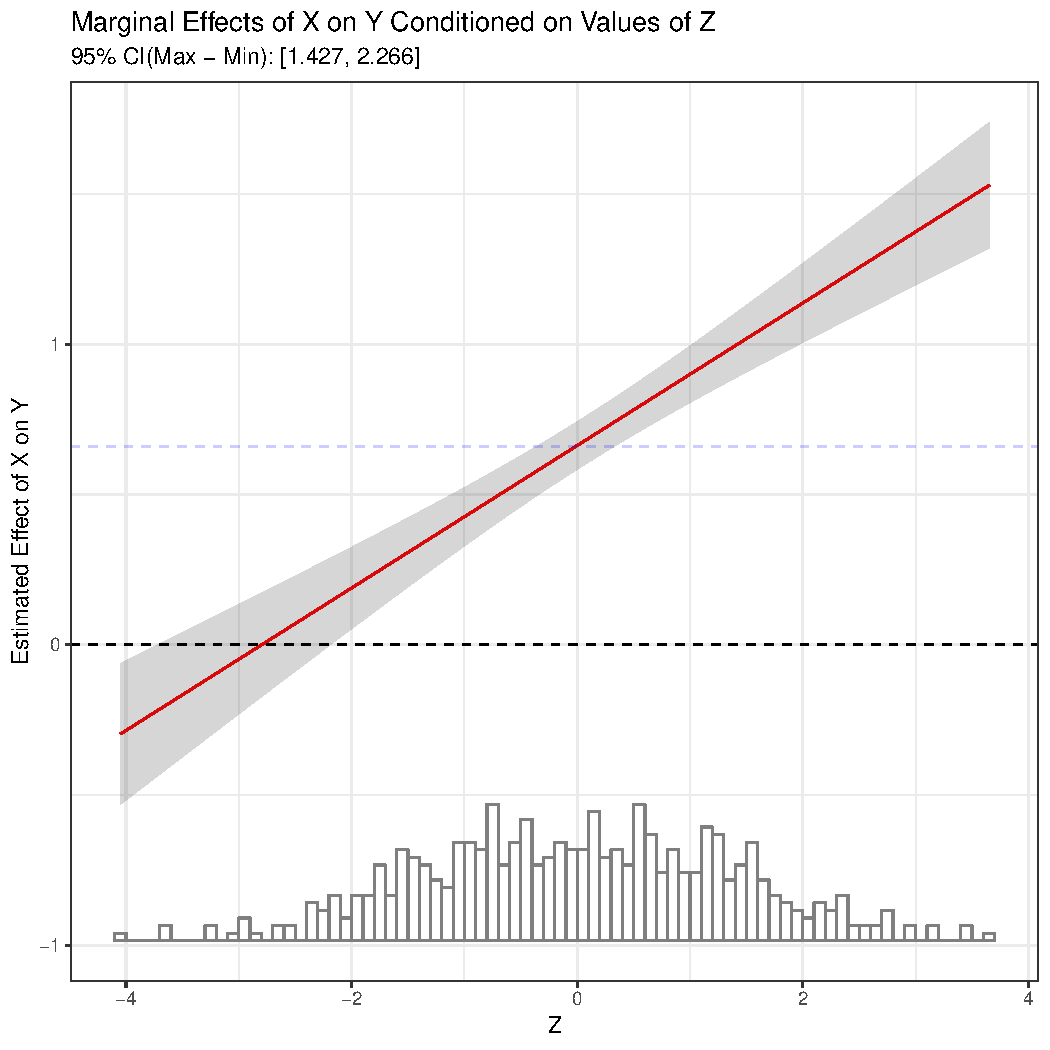
\includegraphics[scale=.6]{images/cond0.pdf}
    \caption{Conditional marginal effects of $X$ on $Y$ across values of $Z$. The red line represents the estimated marginal effects, with the gray bands being $95\%$ confidence intervals. The faint blue line at $Y = .66$ shows the estimated marginal effect when the interaction term is not included in the model.}
    \label{fig:cond0}
\end{figure}

Figure \ref{fig:cond0} helps us gain a more comprehensive understanding of how $Z$ moderates the effect of $X$ on $Y$. First, as per equations \ref{mod} and \ref{mod2}, the unstandardized estimate of the interaction effect is equal to the slope of the line observed in the plot $(\hat{\beta}_3 = 0.24)$. Additionally, the marginal effect conditioned on $Z = 0$ is equal to the unstandardized main effect of $X$ on $Y$ $(\hat{\beta}_1 = 0.66)$. The gray bands surrounding the marginal effects represent $95\%$ confidence intervals based on the standard errors estimated from equation \ref{margse}. We can see that the intervals do not include $0$ over most the range of $Z$, and reveal that $X$ is expected to have a significant \textit{negative} effect on $Y$ at low values of $Z$, but a significant \textit{positive} effect across the majority of $Z$'s range. Moreover, the histogram at the bottom of the plot displays the distribution of $Z$, and the $95\%\ \text{CI}$ at the top represents the difference between effects estimated at its maximum and minimum using data simulated from the posterior distribution of $(\hat{\beta}_1 + \hat{\beta}_3 Z)$ with the \code{sim} function from the \code{arm} package in R \cite{arm}. 

\subsubsection{Discussion}
The purpose of this example is to demonstrate how a researcher might go about probing an interaction effect by examining the conditional effects of an independent variable across the range of a continuous moderator. Importantly, this plot illustrates the necessity of testing interaction effects when one is investigating a conditional hypothesis. Although this is a simulated example, we can clearly see that without modeling the interaction between $X$ and $Z$, one's understanding of the relationship between $X$ and $Y$ would be greatly misrepresented. Had the interaction effect not been included, the estimated marginal effect of $X$ on $Y$ would be captured by the dashed blue line where the $y$-axis equals $0.66$. This is the main effect of $X$ on $Y$ in the non-interaction model, where $Z$ is still included as a covariate. The bottom line is that visualizing the character of how two variables interact is crucial for understanding how they might relate with an outcome of interest. Especially for multivariate models such as psychological networks, failing to include relevant interaction terms can lead to misspecified models that improperly characterize the relationships among a set of variables. This plotting function is included as part of the \code{modnets} package for assessing interaction effects within psychological network models; thus, it is a tool that researchers studying moderated networks in psychology will be able to use as part of their analyses and profitably employ to explore the nature of interaction effects in their models. 

\subsection{Summary}
The goal of the present section was to provide a background describing moderation analysis, interaction effects, and how rich information about multivariate relationships can be gained from studying the conditional effects of a given predictor on an outcome after considering values of a moderator. The central point here was to showcase a simple way of extracting this type of information from a moderated regression model to better understand the nature of the relationships among variables.

In the next section, I will present my approach to analyzing \textit{moderated network models}, which are essentially a multivariate generalization of the basic template presented here. Combined with techniques from graphical modeling, adding interaction terms to network models contributes a potentially powerful framework for investigating more complex models and more specific hypotheses (namely, those dealing with moderation and interaction effects). Furthermore, generalizing the concept of plotting conditional effects across values of a moderator, I will present a new contribution to psychological network modeling which I term \textit{conditional networks}. As in the case of plotting marginal effects at specific values of a moderator, I will show how we can construct networks after conditioning on specific values of a moderator. This offers a way of gaining added information about moderated networks and visualizing the results in easily interpretable plots. I present the basic ideas behind moderated networks in the next section.

\chapter{Moderated Network Models}
The goal of this section is to provide an overview of Moderated Network Models (MNMs) along with some examples of how they can be used to analyze psychological data.
I limit the present discussion to \textit{cross-sectional} MNMs, where the objective is to estimate an undirected network from a sample of $n > 1$ subjects measured on $p$ variables at a single time point. Temporal formulations of these models (i.e., MNMs applied to time series data; both in idiographic and multi-subject settings) will be examined in a separate paper. 

Currently, the MNM framework I present here and implement in the \code{modnets} package supports the analysis of both continuous and binary variables, where each type can serve as either a predictor or an outcome. The simplest case, however, is based on the Gaussian Graphical Model (GGM), wherein all outcomes (i.e., nodes in the network) are assumed to be continuous variables with a multivariate normal distribution. An undirected network consisting of all binary variables is commonly referred to as an \textit{Ising Model}, and has been studied at great length in previous work \cite{lauritzen1996graphical,van2014new,marsman2018introduction}. Moreover, Mixed Graphical Models---where outcome variables may be associated with different univariate distributions---have also received treatment within the literature \cite{yang2014mixed,chen2014selection}. Importantly, all of these models can be formulated as MNMs using the same basic approach, although the results will be subject to different interpretations and are not necessarily associated with a normalizable joint distribution \cite{yang2014mixed, haslbeck2018moderated}. In such cases, this precludes us from computing the likelihood of the model when taken as a whole, thereby preventing us from performing global goodness-of-fit analyses along with model comparison tests. Thus, to outline the basic foundation of MNMs here, I focus on the scenario where all outcome variables are assumed to be continuous, Gaussian variables, as these have the most straightforward interpretation along with a normalizable joint distribution. 

I distinguish between two different types of MNMs: (a) the \textit{exogenous} MNM, and (b) the \textit{endogenous} MNM. The qualifier in each case is meant to refer to the nature of the moderator variable(s) included in the model. For an \textit{exogenous} MNM, we essentially treat the moderator variable(s) as covariates in the model; that is, they are not treated as outcomes which are affected by the other variables, and therefore are not represented as nodes in the resulting network. Instead, they are treated as external components of the process or system under investigation. Identification of moderators as exogenous variables should be based on theory, or based on a reasonable assumption that the variable in question is not influenced by the other variables under study (such as ethnicity, experimental condition, gender, etc.). With \textit{endogenous} moderators, however, these variables will be identified as nodes in the network and treated as outcomes in the construction of the model. This latter case will be most useful in exploratory settings, and will be discussed in a separate paper. Thus, in the remainder of this section I will present the foundation for estimating and interpreting MNMs wherein all outcomes are Gaussian variables and there is only one moderator which is treated as an exogenous variable.

\section{Estimation}
The standard way of constructing a GGM is through joint estimation of model parameters via the standardized inverse covariance matrix---i.e., the \textit{partial correlation matrix}. Let $\bX$ be an $n \times p$ matrix, where each column represents a different variable $(j = 1,\ldots,p)$, and each row contains the response vector for a single subject $(i = 1,\ldots,n)$. For the standard GGM, we assume that the response vectors are multivariate normal:
\begin{equation} \label{mvn}
    \bx_i \sim \N(\bmu, \bSigma)\ \forall i\in\{1,\ldots,n\},
\end{equation}
where $\bmu$ is the $p \times 1$ vector of means, and $\bSigma$ is the $p \times p$ variance-covariance matrix. For simplicity, we will also assume that all the variables have been mean-centered, such that $\bmu = \matr{0}$. Thus, our only objective is to estimate the partial correlation matrix $\bOmega$, which is a $p \times p$ symmetric matrix with zeros in the diagonal and partial correlations between each pair of variables in the off-diagonal. This can be obtained by taking the maximum likelihood estimate (MLE) of $\bSigma$ and standardizing its inverse (i.e., the precision matrix), such that
\begin{equation} \label{ggm}
    \hat{\bSigma} = \frac{\bX\tran\bX}{n},\quad\text{and}\quad \hat{\bOmega} = \I - \bDelta \hat{\bSigma}\inv \bDelta,
\end{equation}
where $\I$ is a $p \times p$ identity matrix, and $\bDelta$ is a diagonal scaling matrix with zeros in the off-diagonal and $\diag{\bDelta} = \diag{\hat{\bSigma}\inv}^{-\frac{1}{2}}$. The resulting estimate of $\bOmega$ therefore encodes the conditional dependence structure of the data, and is used to define the undirected network. 

When moderators, covariates, or any higher-order interaction terms are included in the model, however, this approach is no longer possible. Instead, we can use an approach called \textit{nodewise regression} \cite{haslbeck2015mgm,epskamp2018gaussian}. This method is based on a graph-theoretic approach to structure learning called neighborhood selection \cite{meinshausen2006high}, and entails estimating the network structure via a series of univariate regression models. That is, a separate regression model is constructed for each variable represented as a node in the network, and then the coefficients are aggregated across models to define the final network structure.

For example, imagine that we wanted to model the conditional dependence of three random variables: $X_1$, $X_2$, and $X_3$. Taking the nodewise regression approach, we would begin by constructing three separate univariate regressions:
\begin{equation} \label{mod0}
    \begin{split}
        X_1 &= \beta_{10} + \beta_{12} X_2 + \beta_{13} X_3 + \eps_1 \\
        X_2 &= \beta_{20} + \beta_{21} X_1 + \beta_{23} X_3 + \eps_2 \\
        X_3 &= \beta_{30} + \beta_{31} X_1 + \beta_{32} X_2 + \eps_3.
    \end{split}
\end{equation}
Given that the slope parameters represent directed conditional relationships---e.g., in this example, $\beta_{12}$ is the slope predicting $X_1$ from $X_2$ after conditioning on $X_3$---we can combine relevant pairs of coefficients to obtain the \textit{undirected} conditional dependencies (i.e., partial correlations) between variables. For instance, here the partial correlation between $X_1$ and $X_2$ can be defined as $\omega_{1,2} = \sign{\beta_{12}}\sqrt{\beta_{12}\beta_{21}}$. It is important to note that the signs of $\beta_{12}$ and $\beta_{21}$ will always be the same if and only if the two slope parameters are conditioned on the same covariates (e.g., $X_3$ serves as a covariate in both models), and $n > p$ \cite{williams2019nonregularized}. 

While this equivalence holds when exogenous covariates are included as predictors in the nodewise regressions, it no longer holds when interaction terms are included. That is, imagine that we included a potential moderator $Z$ in the current example. We would now have the following equations:
\begin{equation} \label{mod1}
    \begin{split}
        X_1 &= \beta_{10} + (\beta_{12} X_2 + \beta_{13} X_3 + \beta_{1Z} Z) + (\theta_{1,2Z} X_2 Z + \theta_{1,3Z} X_3 Z) + \eps_1 \\
        X_2 &= \beta_{20} + (\beta_{21} X_1 + \beta_{23} X_3 + \beta_{2Z} Z) + (\theta_{2,1Z} X_1 Z + \theta_{2,3Z} X_3 Z) + \eps_2 \\
        X_3 &= \beta_{30} + (\beta_{31} X_1 + \beta_{32} X_2 + \beta_{3Z} Z) + (\theta_{3,1Z} X_1 Z + \theta_{3,2Z} X_2 Z) + \eps_3.
    \end{split}
\end{equation}
Here I use parentheses to separate main effect terms from interaction terms, where parameters associated with main effects are represented by $\beta$ and those associated with interactions are represented by $\theta$---this distinction is purely for notational clarity.

In these cases, we cannot directly aggregate main effect parameters and transform them into partial correlations. However, we can still approximate the conditional dependencies between variables by averaging over relevant pairs of coefficients; this is a common approach taken in the psychological network literature, even when interactions are not included and exact partial correlations could otherwise be computed \cite{haslbeck2015mgm,epskamp2018gaussian}. While this approach seems simple enough, the examples I've provided so far exemplify cases where each nodewise regression is saturated with all possible terms. In practice, however, model selection procedures are often implemented to determine whether or not all terms should be included in the final models. 

For example, perhaps we find that $X_2$ strongly predicts $X_1$, and so we estimate $\beta_{12}$. But, based on theory or some model selection procedure we conclude that the converse is not true (i.e., $X_1$ is not an important predictor of $X_2$), and so opt to exclude $\beta_{21}$ from the final set of models. This means that we implicitly assume $\beta_{21} = 0$. Now we must choose whether to draw an edge between $X_1$ and $X_2$ in the resulting network. It is common to make this decision by employing either the `AND' or `OR' rule: with the `AND' rule, we only draw an edge between $X_1$ and $X_2$ if both $\beta_{12}$ and $\beta_{21}$ are estimated to be non-zero, whereas with the `OR' rule we draw an edge between the two nodes if at least one of the two relevant parameters is non-zero. In the current example, the edge between $X_1$ and $X_2$ would be calculated as $(\beta_{12} + 0)/2$. 

\section{Analyzing Moderated Networks}
It will be helpful to use an example that illustrates the process of analyzing moderated networks. For simplicity, I will use a subset of the \code{msq} dataset from the R package \code{psych} \cite{psych}. The data consist of $n = 3896$ responses to 75 items on the Motivational State Questionnaire, which measures a variety of mood states on scales ranging from $0$ to $3$. While these variables are clearly ordinal rather than continuous, I chose these data because they resemble a common scenario in psychological research. For this example I will only focus on $5$ items from the questionnaire: \textit{hostile}, \textit{lonely}, \textit{nervous}, \textit{sleepy}, and \textit{depressed}. Here, we will treat \textit{depressed} as an exogenous moderator variable, and will investigate whether the relationships among the other $4$ mood states vary across levels of depression. 

\subsection{Visualization}
First, we begin by mean-centering the data. Although given that $0$ is a value on the scales, it could be argued that mean-centering is not necessary in this case. Nevertheless, centering allows us to assess the relationships between variables at their mean levels, and also reduces the correlations between multiplicative terms and their constituents \cite{lance1988residual,brambor2006understanding}. The next step is to fit $4$ nodewise regressions, one for each of the $4$ outcomes: \textit{hostile}, \textit{lonely}, \textit{nervous}, and \textit{sleepy}. Each regression therefore contains $7$ predictors, with $4$ main effects and $3$ interaction terms. Upon aggregating the coefficients we obtain the following plot.

\begin{figure}[htbp]
    \centering
    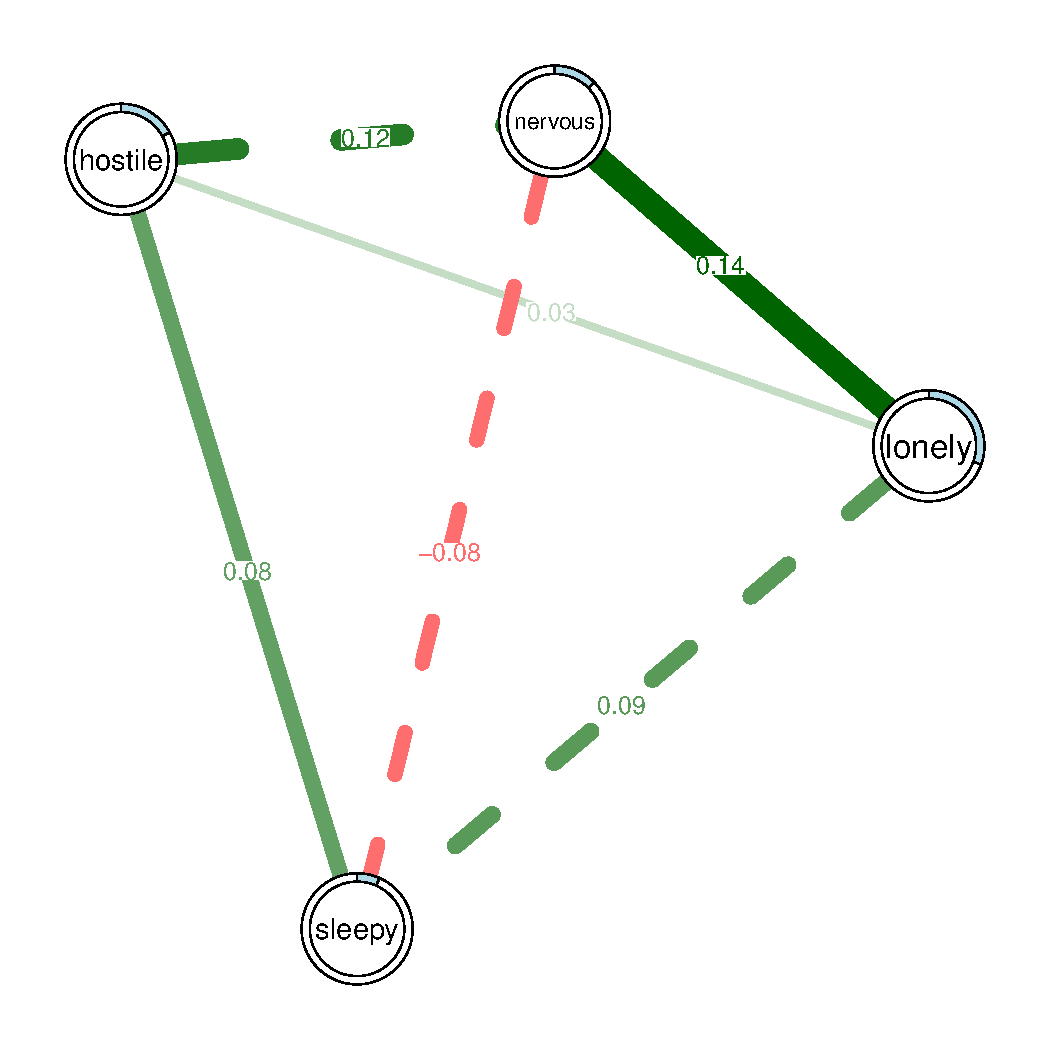
\includegraphics[scale=.6]{images/plot1.pdf}
    \caption{Moderated network model at \textit{depressed} $= 0$, plotted with the AND rule and all interaction terms included in each nodewise regression.}
    \label{fig:plot1}
\end{figure}

In Figure \ref{fig:plot1}, green lines indicate a positive relationship between two variables, red lines indicate negative relationships, and dashed lines indicate that the relationship between two nodes is moderated by the \textit{depressed} variable at $p < .05$. Here the coefficients have been aggregated using the AND rule. Given that all models are saturated, applying either the AND or OR rule produces the same aggregated parameters. However, the rule also determines whether a dashed line is used to indicate the presence of moderation effects---specifically, when using the AND rule I only use a dashed line if \textit{both} relevant interaction terms pass a threshold for significance, while for the OR rule I would draw a dashed line if \textit{at least one} of the two relevant interactions pass the threshold. 

To elaborate, here the interaction term \textit{nervous} $\times$ \textit{depressed} is a significant predictor of \textit{hostile}, and the interaction \textit{hostile} $\times$ \textit{depressed} is a significant predictor of \textit{nervous}. Thus, a dashed line is drawn between the two corresponding nodes in the network. Conversely, the interaction \textit{sleepy} $\times$ \textit{depressed} is a significant predictor of \textit{hostile}, but \textit{hostile} $\times$ \textit{depressed} is not a significant predictor of \textit{sleepy}. So, using the AND rule, the edge between \textit{hostile} and \textit{sleepy} is represented with a solid line, given that only one of the two relevant interaction terms are significant---this edge would be drawn as a dashed line if we chose to apply the OR rule instead. 

\subsection{Visualizing the exogenous moderator}
The \textit{depressed} variable is not represented in the overall network because it is not being considered as an outcome. However, this variable still serves as a predictor in all $4$ regression equations. Thus, we can choose to visualize this variable as an exogenous node in the network as well. In Figure \ref{fig:plot2}, I use a square to represent \textit{depressed} along with arrows denoting its links to the other variables to indicate that this variable only serves as a predictor and is therefore conceptualized as being external to the network. This same approach is taken when other exogenous covariates are included in the model, even if they don't serve as potential moderators.

\begin{figure}[htbp]
    \centering
    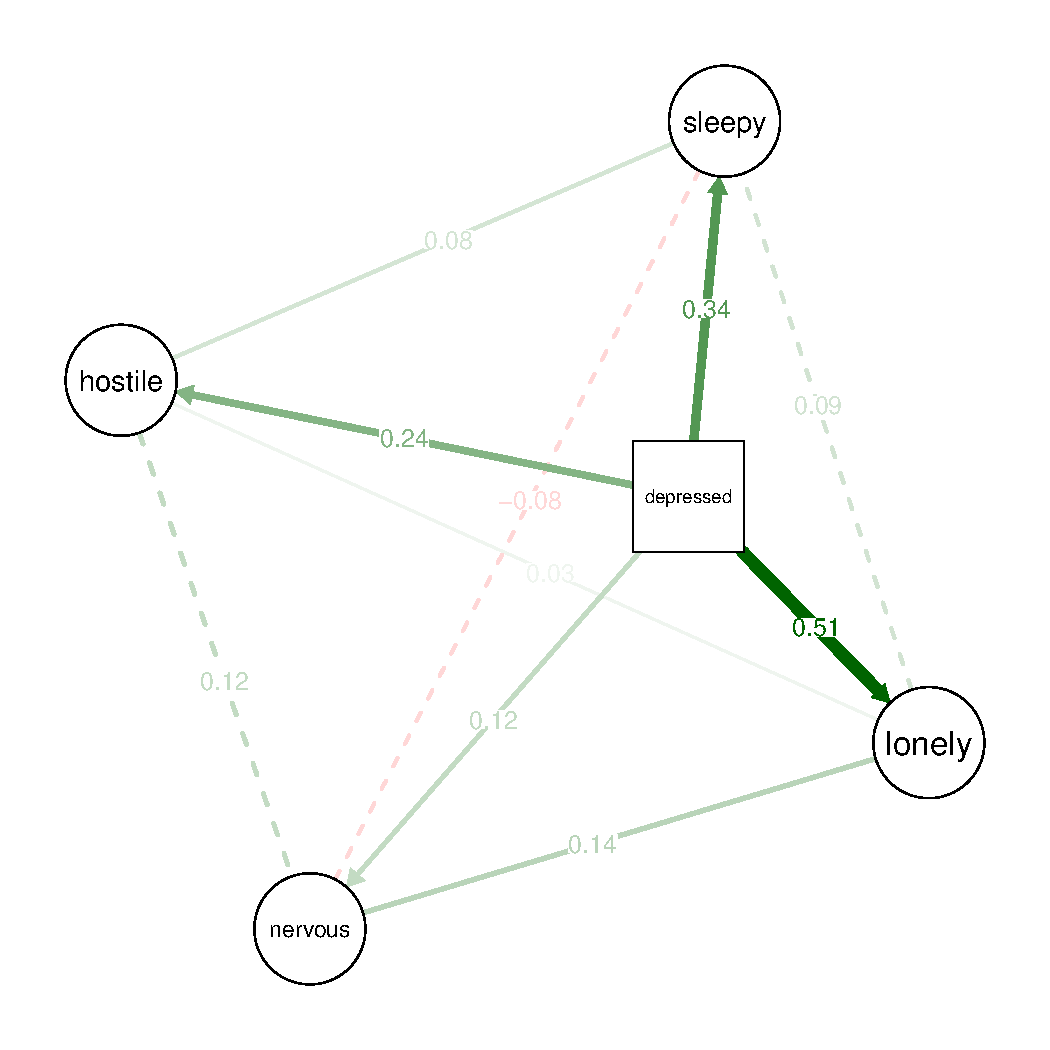
\includegraphics[scale=.6]{images/plot2.pdf}
    \caption{Moderated network model with the exogenous moderator plotted. The color saturation of the edges is scaled against the largest edge weight, which is represented by the beta weight of \textit{depressed} on \textit{lonely}.}
    \label{fig:plot2}
\end{figure}

\subsection{Conditional networks}
Given that there are interaction effects in these models, we cannot interpret the network as representing average or overall conditional dependencies between variables. Instead, these values denote the conditional dependencies between nodes when \textit{depressed} $= 0$; which, since all of the variables have been mean-centered in this example, is equal to the sample mean of \textit{depressed}. The dashed lines in Figures \ref{fig:plot1} \& \ref{fig:plot2} then show us which relationships we should expect to vary across levels of the moderator, while solid lines show us which relationships we should expect to remain constant. Thus it is important to investigate how the network changes across different levels of the moderator, in order to gain more detailed insights into the nature of the interaction effects.

For this example, we will look at how the network changes at increasing levels of depression. That is, using equations \ref{marg} \& \ref{margse} we can compute marginal values of the slope parameters (along with their corresponding standard errors) after conditioning on fixed values of the \textit{depressed} variable (i.e., conditional effects). This is the same approach taken in standard moderation analysis when, given a continuous moderator, researchers often visualize slopes at mean levels of the moderator as well as at $+/-1$ \textit{SD}. Given that the \textit{depressed} variable is positively skewed in this case, however, we will instead compute marginal slopes for the values \textit{depressed} $\in \{0,1,2\}$.

\begin{figure}[htbp]
    \centering
    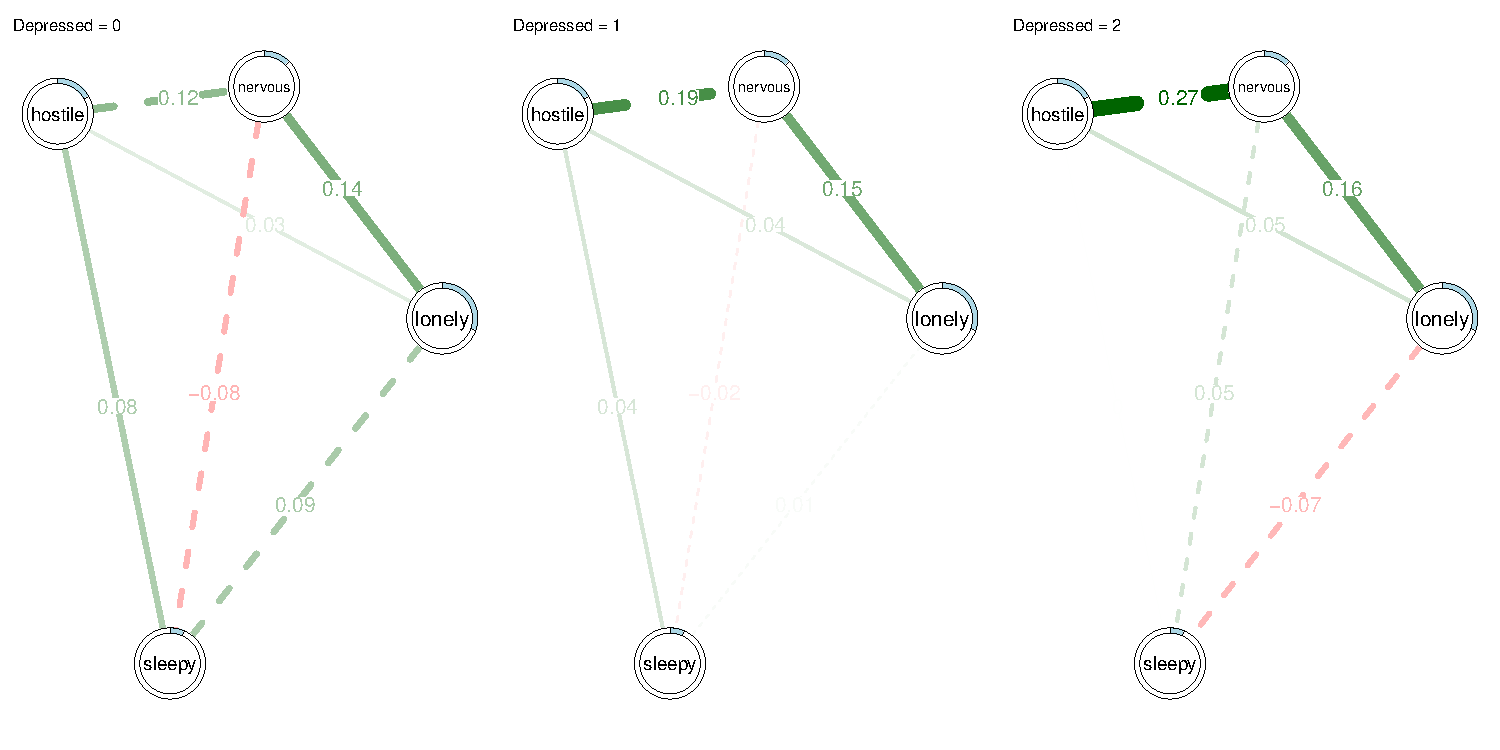
\includegraphics[scale=.6]{images/plot3.pdf}
    \caption{Conditional network models at the values of \textit{depressed} $\in \{0,1,2\}$. Plotted with the AND rule and no significance thresholding.}
    \label{fig:plot3}
\end{figure}

I refer to the plots in Figure \ref{fig:plot3} as \textit{conditional networks} to indicate that they exhibit relationships between variables after conditioning on fixed values of the moderator. In fact, any time we include interaction terms in these models we will always have a conditional network. You'll notice that the first network here is identical to the one previously shown; this is because including interaction terms implicitly means that all constituent main effects represent the slopes when the moderator equals $0$. The only difference between the two visualizations lies in the width and saturation of the edges, as those in the conditional networks plotted in Figure \ref{fig:plot3} are scaled against the largest edge weight, which is the edge connecting \textit{hostile} and \textit{nervous} in the network where \textit{depressed} $= 2$. 

Lastly, while thus far the AND rule has only determined whether or not edges are drawn with a dashed or solid line (based on the presence of significant interaction terms), we can similarly apply the thresholding rule to all model parameters. That is, we can determine whether to draw an edge between two nodes based on whether the main effect terms are significant at some threshold (here, $p < .05$). Using the AND rule, we determine that an edge is drawn between two nodes if both relevant main effects are significant at this cutoff. Thus, in Figure \ref{fig:plot4}, we have a set of networks that only represent the most important relationships between variables, in addition to the most important interaction effects.

\begin{figure}[htbp]
    \centering
    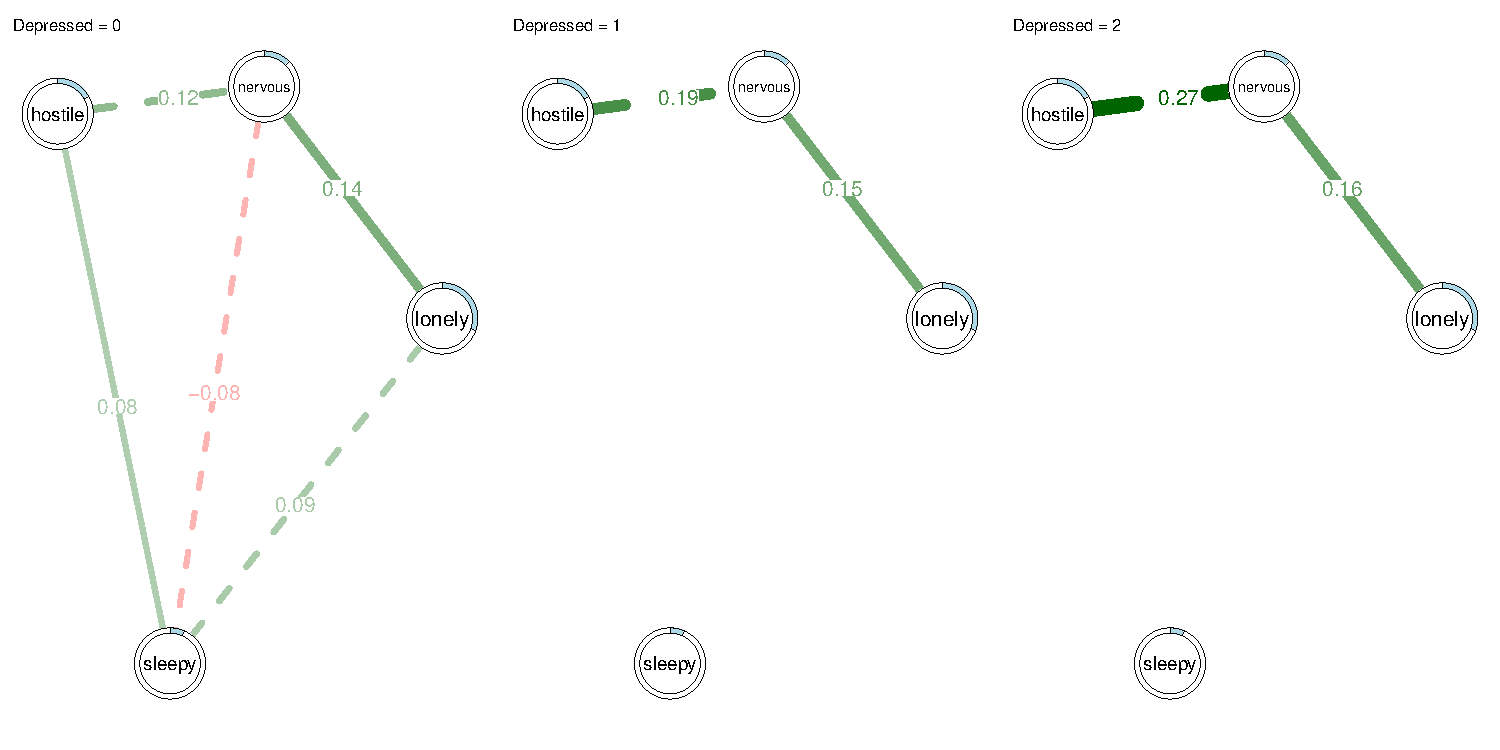
\includegraphics[scale=.6]{images/plot4.pdf}
    \caption{Conditional network models at the values of \textit{depressed} $\in \{0,1,2\}$. Plotted with the AND rule and a significance threshold of $p < .05$.}
    \label{fig:plot4}
\end{figure}

\subsection{Interpreting results}
We can now more clearly see how the network structure changes at increasing levels of depression. Looking only at the plots where thresholding was applied (i.e., Figure \ref{fig:plot4}), we can see that only two relationships persist across levels of depression: (a) that between \textit{nervous} and \textit{hostile}, and (b) between \textit{nervous} and \textit{lonely}. Moreover, we can see that the latter relation remains relatively constant across levels of depression, spanning $\lbrack .14, .16\rbrack$, while the former relation exhibits a significant increase as depression increases, as reflected by the significant interaction effects that modulate the strength of the edge. 

At low levels of depression, we see some other significant, yet small, relationships: (a) a positive relationship between \textit{hostile} and \textit{sleepy}, (b) a positive relationship between \textit{sleepy} and \textit{lonely}, and (c) a negative relationship between \textit{nervous} and \textit{sleepy}. None of these relationships breach our significance threshold at higher levels of depression. The latter two edges appear with dashed lines, however, indicating that they are significantly moderated by levels of depression. We can get a clearer sense of what this means by looking at the non-thresholded set of models in Figure \ref{fig:plot3}. Specifically, both of these relationships switch signs at higher levels of depression, although they do not reach significance in those models. 

If we want to hone-in on any of these results more specifically, we can also look at the marginal changes in the slopes across levels of the moderator, in terms of conditional marginal effects plots. In Figure \ref{fig:conds}, we can clearly see how the relationship between \textit{hostile} and \textit{nervous} increases as depression increases, as well as how the signs of the aforementioned relationships change across this range as well. Lastly, some limitations of this investigation are made clearer in these marginal effects plots. 

\begin{figure}[htbp]
    \centering
    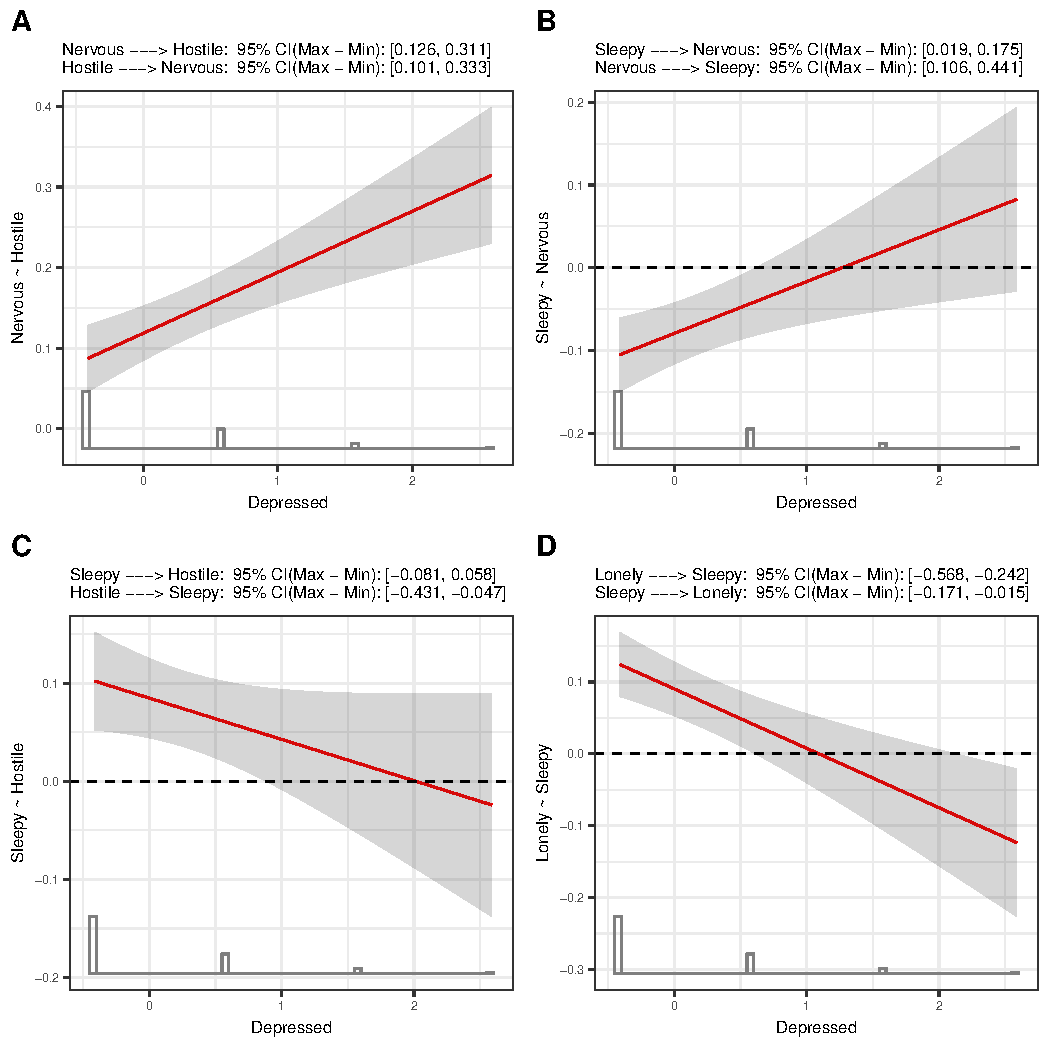
\includegraphics[scale=.7]{images/conds.pdf}
    \caption{Four plots of conditional marginal effects. Each plot represents average values across both relevant interaction terms. In (A), the plot shows the average of two separate conditional marginal effects: that of \textit{hostile} $\times$ \textit{depressed} on \textit{nervous}, as well as for \textit{nervous} $\times$ \textit{depressed} on \textit{hostile}. In (B), the plot shows the average of the conditional marginal effects of \textit{sleepy} $\times$ \textit{depressed} on \textit{nervous}, as well as for \textit{nervous} $\times$ \textit{depressed} on \textit{sleepy}. In (C), the plot shows the average of the conditional marginal effects of \textit{sleepy} $\times$ \textit{depressed} on \textit{hostile}, as well as for \textit{hostile} $\times$ \textit{depressed} on \textit{sleepy}. In (D), this is the average conditional marginal effects of \textit{lonely} $\times$ \textit{depressed} on \textit{sleepy} and \textit{sleepy} $\times$ \textit{depressed} on \textit{lonely}.}
    \label{fig:conds}
\end{figure}

First, the distribution of the \textit{depressed} variable is highly right-skewed; there are a large number of observations at low levels of depression, with fewer and fewer observations as levels of depression increase. Second, the ordinal nature of this variable is made very apparent in the histograms at the base of these plots. Thus, the treatment of this variable as continuous---both in the marginal effects plots and in the analysis---seems somewhat dubious. It would be more appropriate to treat the $4$ possible responses as discrete, ordered categories, at least based on the available sample values. Lastly, the values $\{0,1,2\}$ are not actually represented within the sample once the variable has been mean-centered, and so it would make more sense to plot networks at the values which are used in the analysis. I only chose the three values here for simplicity in this demonstration.

\subsection{Summary}
The goal of this section was to demonstrate a very basic analysis using the moderated network framework. We can see in this example that it is not enough to simply examine one network to understand the conditional dependencies among variables that are subject to interaction effects. Plotting and investigating conditional networks is a crucial part of the analysis, and can reveal patterns in the data that highlight which relationships are most important, which ones change across levels of the moderator, and which relations only emerge under certain conditions (e.g., low values of depression). Continuing with the present example, I will discuss goodness-of-fit indices and model comparison functions that further expand on this type of investigation.

\section{Model Comparison}
Beyond analyzing specific properties of the variables' conditional dependence structure, procedures for model comparison and variable selection (in this case, edge-selection) are important to determine whether or not interaction effects are valuable for the models, as well as whether more parsimonious models with fewer edges can be specified without sacrificing explanatory power. Luckily, when standard estimation procedures are used (as in the current example), standard fit indices and model comparison tests can be employed. There are two levels at which these indices can be assessed: (a) nodewise, and (b) global model fit. 

\subsection{Nodewise Fit Measures}
In the case of models where all outcome variables are assumed to be continuous, we can calculate measures of predictive accuracy for each of the nodewise regressions such as $R^2$, and $R_{adj}^2$ to determine the proportion of the response variance accounted for by the predictors overall, as well as after controlling for the number of predictors (respectively). Additionally, we can assess model fit by computing the log-likelihood, which for a continuous outcome $\bx^{(j)}$ is
\begin{equation}
    \ell(\hat{\bbeta},\hat{\sigma^2}\,|\,\bX) = -\frac{n}{2}\log(2\pi) - \frac{n}{2}\log(\hat{\sigma}^2) - \frac{1}{2\hat{\sigma}^2}\sum_{i=1}^n (x_i^{(j)} - \bx_i^{(-j)}\hat{\bbeta})^2,
\end{equation}
where the superscript $^{(j)}$ indicates the $j$th outcome variable, and $^{(-j)}$ denotes the set of columns from the design matrix (here, $\bX$) that excludes the $j$th variable. The predicted values of $\bx^{(j)}$ are therefore defined as the dot product $\hat{\bx}^{(j)} = \bX^{(-j)}\hat{\bbeta}$, and the MLE for the residual variance is $\hat{\sigma}^2 = \frac{1}{n}\sum_{i=1}^n (x_i^{(j)} - \hat{x}_i^{(j)})^2$. 

Using $\ell(\hat{\bbeta},\hat{\sigma^2}\,|\,\bX)$ we can then compare one model of $j$ (perhaps one including interaction terms) with another by performing a \textit{likelihood ratio test} (LRT), or by computing other fit indices such as the AIC and BIC. These information criteria are defined as
\begin{equation}
    \text{AIC} = 2k - 2\ell(\hat{\bbeta},\hat{\sigma}^2\,|\,\bX),\quad\text{and}\quad\text{BIC} = k\log(n) - 2\ell(\hat{\bbeta},\hat{\sigma^2}\,|\,\bX),
\end{equation}
with $k$ being the number of parameters estimated in the model. The AIC and BIC are transformations of the log-likelihood that afford different emphases in the model selection process by penalizing models with a larger number of parameters. The BIC enforces a stronger penalty than the AIC on models with a greater number of parameters, and is thereby the more conservative of the two \cite{yang2005can}. These criteria are particularly important when we have a large number of variables to consider, or are especially concerned with preserving model fit while limiting ourselves to select a more parsimonious model. 

In the \code{modnets} package, all of these criteria are made available to assess model fit. Nodewise LRTs can be conducted to compare models for each node, individually, across different specifications of the network, and indices of predictive accuracy---namely, $R^2$ and $R_{adj}^2$---can be depicted graphically to accompany the network representations. This approach was first used by \cite{haslbeck2017predictable}, but has been expanded in the \code{modnets} package to allow for model comparison. For instance, in Figure \ref{fig:plot5} we visualize the same model as in Figure \ref{fig:plot1}, but use blue rings around each node in (A) to denote the $R^2$ value of each model in comparison with a model that excludes the interaction terms, as well as the \textit{depressed} variable. Specifically, the light blue represents the $R^2$ of the reduced model (excluding interaction terms and the \textit{depressed}) variable, while the darker blue represents the additional $R_{\Delta}^2$ that is contributed by including \textit{depressed} and the accompanying interaction terms. 

\begin{figure}[htbp]
    \centering
    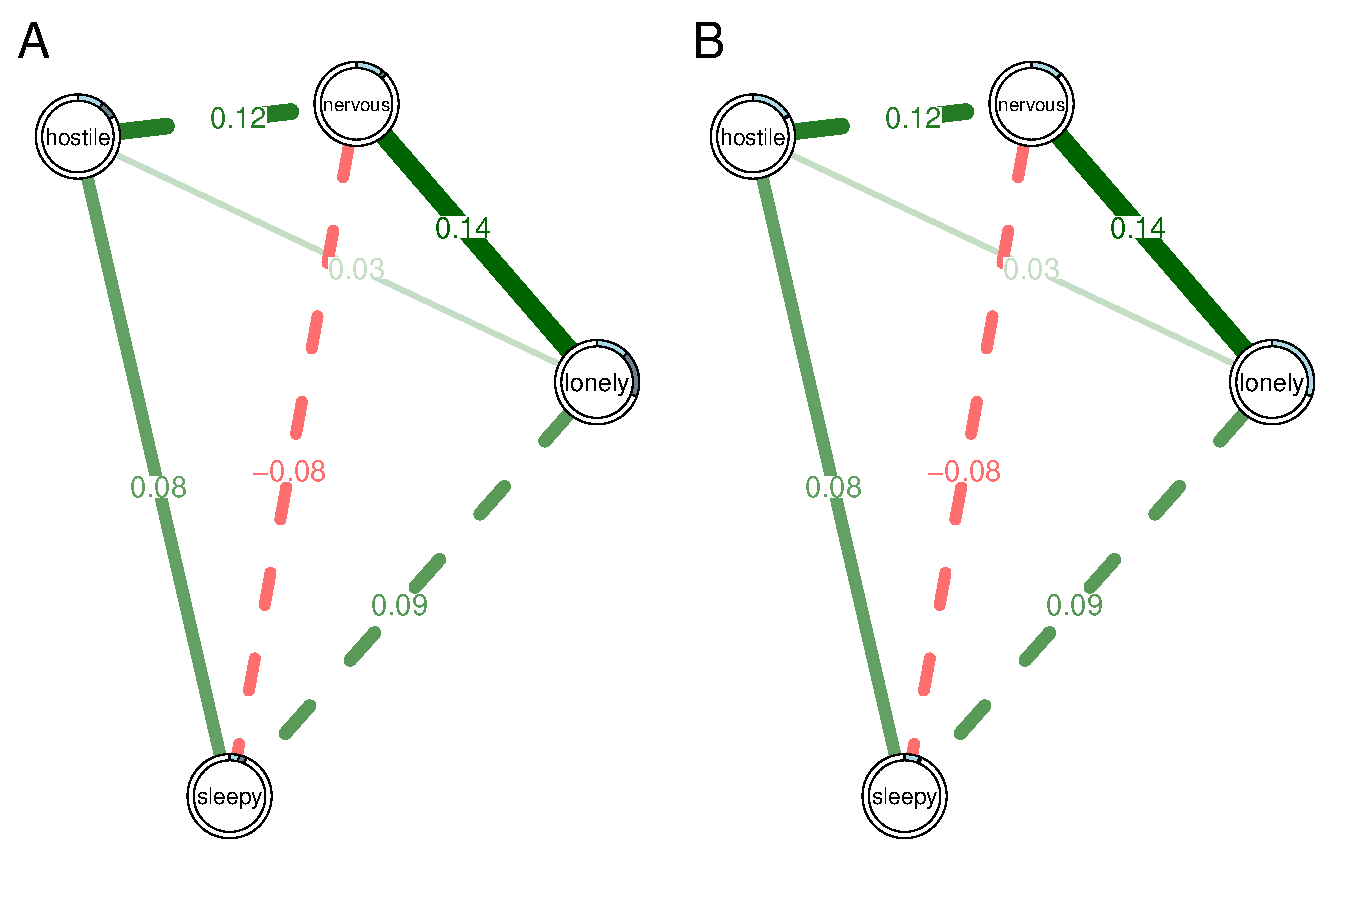
\includegraphics[scale=.6]{images/plot5.pdf}
    \caption{These plots show the same network model as in Figure 2, but with two different comparisons represented by the blue shading in each node. In (A), the light blue shading represents the $R^2$ for each nodewise regression where \textit{depression} is not included in any of the models, while the dark blue shading shows the $R_{\Delta}^2$ given the models including \textit{depression} as well as all of its interaction effects. In (B), the models being compared to the moderation models include \textit{depressed} as a covariate.}
    \label{fig:plot5}
\end{figure}

When we include \textit{depressed} as a covariate, however, we can now see that the increase in $R^2$ after including the interactions is very small (B). This highlights the importance of using fit indices in addition to these metrics in order to determine which model should be interpreted.

\subsection{Global Fit Measures}
It is possible to obtain similar fit measures to describe the fit of all nodewise models taken together. That is, in certain circumstances we can compute the multivariate log-likelihood as well as the corresponding AIC and BIC values to assess global fit across models. This is currently only possible when all outcomes are continuous and assumed to be multivariate normal. However, even this may be undefined in certain cases when many interaction terms are included, particularly when this prevents the residual covariance matrix from being positive definite \cite{yang2014mixed,haslbeck2018moderated}. The multivariate normal log-likelihood can be written as
\begin{equation}
    \ell(\hat{\bX}, \hat{\bSigma}\,|\,\bX) = \sum_{i=1}^n -\frac{m}{2}\log(2\pi) - \frac{1}{2}\log(|\hat{\bSigma}|) - \frac{1}{2}(\bx_i - \hat{\bx}_i)\hat{\bSigma}\inv(\bx_i - \hat{\bx}_i)
\end{equation}
where $m$ is the number of nodewise regression models being estimated (which may be different from $p$, the number of variables, e.g. when the moderator is exogenous), $\hat{\matr{M}}$ is an $n \times m$ matrix containing the predicted values for each nodewise regression, $\hat{\bSigma}$ is the $m \times m$ residual covariance matrix, and $|\hat{\bSigma}|$ is its determinant.

The global AIC and BIC can also be calculated from $\ell(\hat{\matr{M}}, \hat{\bSigma}\,|\,\bX)$, where we supplant $k$ with $k^*$ to denote the number of estimated parameters summed across \textit{all} nodewise models. From here, we can conduct global LRTs and use the other fit indices to compare network models taken as a whole.

In sum, we can use both nodewise fit measures along with global fit measures to optimize information criteria at each level of analysis and select the best model in accordance with our (the researcher's) priorities. In each of these cases, however, I am assuming that there is a clear set of candidate models for us to consider. In the present example, I've presented $3$ clear candidate models: (a) the set of models excluding \textit{depressed}, (b) the set of models including \textit{depressed} as a covariate, and (c) the set of models including \textit{depressed} and its associated interaction terms as covariates. Yet, it may not always be this easy, as we may have many more variables to consider, or may be conducting an even more exploratory analysis wherein the goal is to assess an array of potential moderators and determine the most parsimonious set of models.

\section{General Discussion}
As psychological network models become more widely used across different areas of research, it is clear that methodological extensions are much needed. One recent approach spearheaded by \cite{epskamp2017generalized} has been to integrate network models with latent variable models in an effort to create `hybrid networks' for studying psychological phenomena. Other new approaches have included networks for time-series models, particularly those that apply to multiple subjects sampled over time \cite{hamaker2018frontiers}, as well as those that use non-parametric, time-varying models to accommodate data that violate parametric model assumptions \cite{bringmann2017changing}. The project described in this paper aims to expand on network models in another, complementary way, and that is by extending current approaches to move beyond strictly pairwise relationships and include higher-order effects such as moderators and interaction terms.

\subsection{Extending Pairwise Networks with Temporal Data}
The central focus of this paper has been on incorporating moderation effects in psychological network models. The present paper focuses exclusively on \textit{cross-sectional networks}, wherein the goal is to study relationships between variables sampled from multiple subjects at a single point in time. The \code{modnets} package is explicitly designed to handle other data types as well---particularly idiographic data, where repeated-measures are analyzed from a single individual, and multilevel data, where multiple subjects are repeatedly measured over time. These will be discussed at greater length in another paper, but for now it can at least be said that the foundations of moderated network models also exist for analyzing repeated, ordered observations, and their implementation in the \code{modnets} package will make it the first available software for analyzing and fitting these types of models.

\chapter{Network Stability and Model Selection}

\begin{enumerate}
    \item Previous chapter focused on how to estimate and interpret moderated network models. But many important questions remain for the researcher hoping to apply such an analysis to their data:
    \begin{enumerate}
        \item Among all possible model structures to choose from, what is the optimal way to decide which model to interpret? That is, on what grounds can we engage in model selection?
        \item Given a model that has been chosen, how can we assess the accuracy of the parameter estimates? More specifically, how can we assess the degree to which our model is subject to sampling variation? (Accuracy = proneness to sampling variation)
        \item How stable is a particular model structure, and how likely is it to replicate in another sample? (Stability -- robust structure in smaller samples)
        \item Finally, how can we address issues of statistical power and determine necessary sample sizes a priori?
    \end{enumerate}
    \item Each of these questions will be dealt with in this chapter and accompanied by simulations to demonstrate various ways of exploring a dataset, designing confirmatory network-based studies, and providing a comprehensive analysis of moderated networks that address common issues/questions in modeling complex networks using real data.
\end{enumerate}

\section{Model Selection}
First step is talking about the importance of selecting a good model. The key is to balance parsimony with predictive accuracy, particularly when this is an out-of-sample based form of accuracy. Researchers who work with psychological networks often make an assumption that the `true' network or `true' model is sparse. This means that researchers typically anticipate that only a moderate to small proportion of the total number of possible relationships in a given network actually map onto real causal connections, rather than spurious associations. The implication of this assumption is that researchers are faced with the often difficult task of determining which model to choose and interpret.

Model selection is certainly not a new statistical problem by any means. In fact it is standard procedure in most situations of modeling multivariate or complex phenomena. Common techniques that have been used for decades include forward, backward, and best-subset selection, all of which involve searching a large probability space and comparing a multitude of models to find which fits some pre-defined criterion (e.g., to minimize the sum of squared errors, or some other information criterion). Overall, we can distinguish between 3 general approaches to model selection: (a) Thresholding (pruning), (b) Model search, and (c) Regularization.

\subsection{Thresholding}
Thresholding is probably the simplest and most widely used form of model selection. The most basic example of this would be when a researcher fits a regression model with multiple predictors, but then only interprets the effect estimates which, under the null hypothesis, are sufficiently low in probability (e.g., $p < .05$). The most common way of implementing this method is by simply restricting one's interpretation of the model to its significant parameters (the threshold of which will be determined by the researcher). Alternatively, one might assess which parameters of a given model are significant and then re-fit the model while only including those parameters. In highly complex models with many variables, however, this routine can be implemented recursively until the researcher cannot add or subtract any parameters on the basis of the pre-defined threshold.

\subsection{Model Search}
Thresholding is a rather crude way of performing model selection, as the researcher commits to making binary decisions about model parameters based on a fixed significance threshold, and therefore does not think cautiously about the effects of including/excluding any given parameter, and whether certain combinations of included parameters lead to unexpectedly well-fitting models. The central question driving \textit{model search} as a model selection process  is: what model explains the data appropriately while also being as simple as possible?

The primary way of answering this question is by selecting an information criterion that reflects some degree of trade-off between parameter accuracy and parsimony, and then evaluating a variety of models on the basis of that criterion to find the one that satisfies some objective. The challenge here, however, becomes the model space (i.e., the space of all possible models which are being searched). For an undirected network model, for instance, there are $2^{p(p - 1)/2}$ possible models given a network with $p$ nodes. This is another common approach, but can become intractable quickly. Procedures such as backward and forward selection arose to cope with (not solve) this issue. 

\subsection{Regularization}
This is perhaps the method that is least frequently used within the psychological sciences, however it is the method that is extremely prominent within the network-modeling community. The downside of thresholding and model search is that estimation and selection are performed in separate steps. First a model is estimated, and then parameters are evaluated as candidates for inclusion/exclusion in the model, and then a new model is fit. With regularization, the idea is to use a different estimator---specifically a \textit{penalized} estimator---such that estimation and variable selection are performed in the same step. This can be achieved via that LASSO, which stands for Least Absolute Shrinkage and Selection Operator. The LASSO is extremely common within the psychological network literature, and is almost a default in the current community.

The upsides of the LASSO is that it is highly efficient and performs automatic variable selection when parameters for a model are estimated. The downsides, however, are that (a) the estimates from the LASSO are fundamentally biased (e.g., all estimates are shrunk closer to, or exactly to, zero), and (b) this prevents proper standard errors from being determined for the estimates; the sampling distribution of a LASSO'd parameter is unknown, and cannot be approximated through bootstrapped resampling. 

\subsection{The Problem with Moderated Networks}
Although these approaches for selecting a model among an array of potential candidates are widely studied and applied to many different problems. However, in the case of higher-order interaction terms (whether these are multiplicative interactions between multiple variables, or polynomial effects e.g., with respect to time), these semi-automated approaches to model selection can be problematic. Specifically, it is widely acknowledged that omitting constituent main effects associated with a multiplicative interaction term when it is included in a model can lead to biased coefficients of the relationships between the predictors and the outcome(s). [COULD BE COOL TO HAVE AN EXAMPLE HERE SHOWING HOW OMITTING MAIN EFFECTS LEADS TO BIASED ESTIMATES].

\subsection{Summary}
Basically, (a) model selection is important, (b) many methods are available, but most of these fall short when it comes to evaluating models with higher-order interactions. What we need are algorithms and methods that enforce a structural hierarchy on the model search and/or regularization process. So, now to introduce the hierarchical LASSO!

\section{Variable Selection with the Hierarchical LASSO}
First, a discussion of the hierarchical LASSO, group LASSO, etc. Then, a deep dive into the algorithms:
\begin{enumerate}
    \item Multi-sample splitting with p-value adjustment
    \begin{enumerate}
        \item Split sample in half. 
        \item Fit hierarchical LASSO on one half
        \item Then, take selected variables from first half and fit unregularized model with those parameters to the second half.
        \item Save estimates from each iteration, but particularly the p-values. If a variable is not selected in a given iteration, set the p-value to 1. 
        \item Finally, use a quantile-based adjustment to the resulting distribution of p-values associated with each parameter in order to control the false discovery rate.
        \item Adjusted confidence intervals can be computed on a similar basis; the final model is then chosen on the basis of either the adjusted p-values or confidence intervals.
    \end{enumerate}
    \item Bootstrapping with p-value adjustment
    \begin{enumerate}
        \item Same shit as above but with bootstrapping... yippee. Although it is interesting to think about what the differences are.. in theory, the subsampling approach should lead to better out-of-sample prediction accuracy, while on the other hand the bootstrapping method would have more power and so may actually generate more stable estimates. [EMPIRICAL QUESTION]
    \end{enumerate}
    \item Stability Selection
    \begin{enumerate}
        \item My favorite version -- simultaneous stability selection. 
        \item This involves undertaking the same multi-sample splitting approach (subsampling), but a separate hierarchical LASSO model is fit to each subsample of the data. Then, for each parameter we assign a 0 or a 1 based on whether or not that variable was selected in both halves of the data.
        \item Once multiple iterations are completed, for each variable we can take the proportion of times that the parameter was chosen in each half of the data across iterations.
        \item Some threshold is determined here... some way to control FDR, but not clear on exactly how to do that.
    \end{enumerate}
\end{enumerate}

It's worth adding that these all act as model selection procedures or algorithms, but in addition to this we must have some criterion on which to base our decisions in the search procedure. This is likely going to be minimizing an information criterion, or minimizing cross-validated error.

%\chapter{Variable Selection in Moderated Networks}
One key assumption in psychological network modeling is that the `true' network has a \textit{sparse} structure. There are two primary reasons for this assumption: (a) First, in many circumstances it seems most likely that there are only a few important (out of many possible) causal pathways among the variables under study, and (b) second, sparse models are much easier to interpret than dense models. The latter point is truly a pragmatic consideration, but is nevertheless important because of the rapidly-increasing degree of complexity in network models as we add new variables to the system (especially when higher-order interactions are included). We need to be able to `hone in' on the key relationships and focus on the primary drivers of a system's behavior in order to better design confirmatory and experimental studies to explore it further. 

Assuming that psychological networks are sparse is often a starting point for network modeling in psychology. This usually seems like a reasonable assumption to make, and it may even be necessary due to the highly exploratory nature of this field of research. Given the large number of relationships that are often being estimated, techniques from machine learning and `big data' come into play more frequently, and thereby bring along new sets of considerations. Specifically, the parameters in network models are often estimated using penalized regression techniques---most notably, the \textit{LASSO}. This approach was designed for high-dimensional data analysis (where $p \gg n$), and offers some notable advantages over other approaches when the goal is to estimate some kind of sparse statistical structure. I will discuss this method in the following sections, as well as some of its drawbacks, and how it can be used in cases where we are interested in studying moderation effects.

\section{Variable Selection with the LASSO}
LASSO is an acronym that stands for `Least Absolute Shrinkage and Selection Operator', and is a method of penalized regression that offers a powerful alternative to ordinary least squares (OLS) \cite{tibshirani1996regression}. The key function of the LASSO is to increase prediction accuracy and model interpretability by shrinking coefficients of the predictors toward zero---importantly, this procedure will often shrink some coefficients to be \textit{exactly} zero, thereby performing automatic variable selection and creating a model that's easier to interpret. The general form of the LASSO can be stated as:
\begin{equation}
    \hat{\bbeta} = \argmin_{\bbeta} \lb \sum_{i=1}^n (y_i - \bx_i \bbeta)^2 + \lambda\sum_{j=1}^p |\beta_j| \rb,
\end{equation}
where $\hat{\bbeta}$ is the vector of coefficients that minimizes the residual sum of squares (RSS) along with an added penalty that weights the sum of the absolute values of the coefficients with a parameter $\lambda$. The objective represented by the formula above could thus be conceptualized as finding the coefficients that minimize: RSS + penalty.

The tuning parameter $\lambda$ governs the strength of the penalty, and thereby the degree of shrinkage that is applied to the coefficients. Larger values of $\lambda$ enforce a larger penalty, which is likely to translate into more parameters being set to zero. At the most extreme, all coefficients may be set to zero, leading to an intercept-only model, and conversely when this parameter is small (or is itself zero), the model will converge toward unpenalized OLS estimates. The optimal value of this parameter is often determined through $k$-fold cross-validation, wherein an array of $\lambda$ values are used in fitting models to different subsets of the data and then tested on $k$ hold-out sets to determine which value results in the lowest cross-validated mean-squared error. Information criteria (such as the AIC and BIC) may be used as an alternative to cross-validation for this purpose, but in all cases the goal is to find which value of $\lambda$ results in the model with the best balance between accuracy and parsimony. 

The primary attractive features of the LASSO are that it narrows down the number of predictors to only the most important (i.e., only those with the strongest relationships to the outcome) by setting the coefficients for some predictors to zero. Not only does this have the advantage of making models more interpretable, but it can also increase prediction accuracy by reducing the possibility of overfitting---that is, fitting a model that gives too much weight to the noise within some particular dataset, and thereby creates a model that fails to generalize well to new cases. 

In the case of modeling psychological networks, these attributes are desirable because of the large number of possible coefficients (`edges') that may be used to describe even a small network. In the most simple case where we are fitting a network model to cross-sectional data, for instance, given $p$ variables (or `nodes') there will always be $p(p - 1)/2$ edges being estimated. When there are only 3 nodes in the network, this means that there will only be 3 edges. But with 6 nodes we now have 15 edges, and with 10 nodes there will be 45 edges. This number grows exponentially as we add more nodes to the network, and is therefore something that researchers aim to minimize as much as possible in order to highlight only the most important relationships. 

\subsection{Disadvantages of the LASSO}
Although the LASSO has some very desirable properties for aiding in interpretation and increasing predictive accuracy, this comes at the cost of producing coefficient estimates that are biased towards zero, and as a result may not provide a good representation of their `true' values. While this is not necessarily a problem when prediction is the goal, it does create a major obstacle for inference. Specifically, there is no known way to determine the standard errors of estimates derived from the LASSO, and thus no way to perform significance tests that can be assumed to reflect the characteristics of the associated sampling distributions. Due to the unique bias of the LASSO estimates (i.e., that it can lead to some parameters being estimated at zero), even bootstrapped resampling fails to be a valid method for determining the distributions of the parameters. This method may be effective when the true coefficients are especially large, or truly equal to zero, but for cases in between it will usually generate asymmetric distributions that may not actually describe the population-level associations between the candidate variable(s) and outcome of interest. 

A related disadvantage of the LASSO, although not unique to the LASSO, is inconsistent model selection. In cases where small changes in the tuning parameter $\lambda$ lead to different variables being included or excluded from the final model, it may be difficult to make strong inferences about the value of those variables for understanding the phenomena under study. To my knowledge, no variable selection technique is immune to this concern, however, and it may be a persistent challenge for any approach of this nature (e.g., best subset selection). However, despite the fact that bootstrapping does not seem to solve the inference problem, it does provide the researcher with a sense of the selection procedure's stability with regard to each of the predictors. One possible way of increasing confidence in the chosen variables is by reporting the selection rates with reference to each predictor; for instance, we may have greater confidence in choosing variables that are selected for the best model within 90\% of subsamples as opposed to those that are chosen only 15\% of the time.


\subsection{Variable Selection and Interaction Terms}
With regard to the current research, it is a problem to employ automatic variable selection when higher-order terms (such as interactions) are included in a model, as they are treated indiscriminately and without regard to their associated lower-order terms. Specifically, this means that models may be selected wherein interaction terms are included without the inclusion of the related main effects. This is problematic, as psychologists are generally interested in determining whether interactions between variables are significant \textit{over and above} the main effects that constitute them. Thus, when interested in assessing the influence of moderator variables on some outcome of interest, it is important to employ a variable selection method that only chooses models which respect the structure of the predictor variables. 

One method that accomplishes this goal is the \textit{hierarchical LASSO}, which was specifically designed for addressing cases of model selection that include higher-order interactions or polynomial terms \cite{lim2015learning,bien2013lasso}. Available approaches that use this method can be specified to only choose models that obey a \textit{strong hierarchy}, meaning that whenever an interaction or higher-order term is selected for a given model, the associated lower-order term(s) are included as well. Two statistical packages that implement this in the R programming language include: \code{hierNet} \cite{bien2013lasso}, and \code{glinternet} \cite{lim2015learning}. Both of these packages utilize an overlapping group LASSO, wherein the LASSO is applied to predictor variables on the basis of their grouping into sets of main effects + interactions, or main effects and their associated polynomial terms. 

Both of these packages produce similar results in a variety of different settings, but \code{glinternet} exhibits a major computational advantage in terms of computing time. Furthermore, while both packages afford researchers to search the entire model space of all possible interactions among all predictor variables, \code{glinternet} also allows one to select a subset of variables (or a single variable) to serve as candidates for interactions. This is particularly useful when the researcher has specific variables in mind which may serve as moderators.

\section{Stability Selection}
Goal is to choose one element from a set of models
\begin{equation}
    \{\hat{S}^{\lambda};\lambda\in\Lambda\}
\end{equation}
where $\Lambda$ is the full set of regularization parameters considered. There might be two problems: (1) First the correct model $S$ might not even be in the set being searched. (2) Second, even if it is a member, it is not clear to know what the ideal values of $\lambda$ would be to detect $S$. With stability selection, we do not simply select one model. Instead the data are perturbed (by subsampling) many times and we choose all structures of variables that occur in a large fraction of the resulting selection sets. 

For a given cut-off $\pi_{\text{thr}}$ with $0 < \pi_{\text{thr}} < 1$ and a set of regularization parameters $\Lambda$, the set of stable variables is defined as 
\begin{equation}
    \hat{S}^{\text{stable}} = \{k:\max\limits_{\lambda\in\Lambda}(\hat{\Pi}_k^{\lambda})\} \geq \pi_{\text{thr}} 
\end{equation}
We keep variables with a high selection probability and disregard those with low selection probabilities. The exact cut-off $\pi_{\text{thr}}$ is a tuning parameter but results vary surprisingly little for sensible choices of the range. Nor do results seem to depend strongly on regularization. Barbieri and Berger (2004) showed predictive optimality results with the \textit{median probability model}, consisting of variables which have posterior probability of being in the model of $\frac{1}{2}$ or greater. This is different than choosing the model with the highest posterior probability. 


\chapter{Moderators in Temporal Networks}
\section{Time Series Models of Psychological Processes}
In order to study psychological processes as they unfold over time, researchers often use repeated sampling techniques, including longitudinal research designs, experience sampling methodology, and ecological momentary assessment. Latent variable models, such as growth curve models and cross-lagged panel models, are often used when few time points are available, but other techniques become available with a greater number of measurements. Specifically, \textit{time series analysis} can be applied when a large number of time points are available, and may afford a richer picture of the temporal dynamics governing intraindividual processes.

\subsection{Stationarity Assumptions}
Strict stationarity requires that all moments of a time series are independent of time---that is, they do not change over time. Second-order stationarity, however, only requires that the first and second order moments are independent of time. For normally-distributed (i.e., Gaussian) time series, all moments beyond the second order moments are fixed, and so second-order stationarity implies strict stationarity. If this is true, then it can be shown that: $\Ev{\by_t} = \bmu_t = \bmu$, which states that the mean does not change over time. Additionally, it must be true that:
\begin{equation}
    \bSigma(\by_t,\,\by_{t-k}) = \bSigma_k = \Ev{(\by_t - \bmu)(\by_{t-k} - \bmu)\tran},
\end{equation}
that is, the auto- and cross-covariances do not depend on occasion $t$ but depend on lag $k$ only, which is the fixed distance between occasions. 

\subsection{Estimating Temporal and Contemporaneous Networks}
In general, temporal networks are directed graphs with weighted edges that signify the magnitude and direction of time-lagged relationships between any pair of nodes. These visualizations essentially summarize the results of a multivariate VAR, wherein each node is regressed onto all other nodes at some time lag, and the resulting beta coefficients from each univariate model define the directed edges along with their weighted values. The contemporaneous network is generally modeled in conjunction with a temporal network, as it characterizes the inverse covariance matrix of the residuals across the different equations. 

\subsubsection{Graphical VAR}
This is the dominant method being used in the network psychopathology literature. First, imagine that you have $T$ repeated measures of $p$ variables for one subject, $n = 1$. The goal is to create a temporal network, which summarizes the time-lagged effects of each variable on every other variable, and then a contemporaneous network which is a GGM consisting of the partial correlations among the residuals of each time-lagged equation. The primary aim is to estimate these two networks together, such that the temporal network shows the lagged effects conditioned on the correlated residuals, and the contemporaneous network shows the relationships that exist once time-lagged effects have been controlled for. Furthermore, the idea behind the GVAR is to apply the LASSO regularization at every step of the way.

In the GVAR procedure, \cite{rothman2010sparse} propose an approach that they call "multivariate regression with covariance estimation' (MRCE). The algorithm starts by fitting intercept-only models in each of the $p$ equations, and then from those estimates (with zeros in place as coefficients for the predictor variables) finding the variance-covariance matrix of the residuals $\hat{\bm{\Sigma}}$. Then, they use penalized maximum likelihood to estimate the coefficient matrix, and the GLASSO to estimate the inverse residual covariances. This goes back and forth until the beta matrix converges to a pre-defined limit. The objective function being minimized is defined as:
\begin{equation}
    (\hat{\matr{B}}, \hat{\bTheta}) = \argmin_{\matr{B},\bTheta} \lb g(\matr{B},\bTheta) + \lambda_1 \sum_{j' \neq j}|\theta_{j'j}| + \lambda_2 \sum_{j = 1}^p \sum_{k = 1}^q |b_{jk}| \rb.
\end{equation}
This essentially follows the process of (1) Starting with a fixed B or Theta (the former may be estimated by separate lasso regressions; the latter may be the error covariance), then estimate either Theta or B (the opposite of what you started with), and repeat until convergence. 

%\apalevelfour{Partial contemporaneous correlations}
The graphical VAR model estimates $\matr{B}$ and $\bTheta$ using a penalized likelihood approach, wherein $\lambda_1$ and $\lambda_2$ are employed as tuning parameters for penalizing the estimates within each matrix. This method uses a criterion-based model selection procedure for choosing optimal values $\lambda_1$ and $\lambda_2$. Then, the strengths of the links in the graphical model are assessed by computing so-called \textit{partial directed correlations} (PDC) and \textit{partial contemporaneous correlations} (PCC) as measures of strength of the lagged and same-time associations between variables, respectively \cite{wild2010graphical}. 

The PCC is defined as the correlation between two variables at the same point in time after removing the linear effects of the other variables at the same point in time and all variables at previous time points. These values are computed based on elements of the estimated residual covariance matrix $\hat{\matr{\Theta}}$. This is the same procedure as constructing a GGM with cross-sectional data.
\begin{equation}
    \text{PCC}(X_{i,t}, X_{j,t}) = - \frac{\hat{\theta}_{ij}}{\sqrt{\hat{\theta}_{ii} \hat{\theta}_{jj}}}.
\end{equation}

%\apalevelfour{Partial directed correlations}
Since the regression coefficients in $\matr{B}$ depend on the unit of measurement, the strength of lagged associations among variables can be measured as PDCs. These values measure the linear association between a dependent variable at time $t$ and an explanatory variable at time $t - 1$ after removing the linear effects of all other variables at time $t-1$. They therefore quantify the direct influence of the explanatory variable on the dependent variable. The PDC is calculated by rescaling the autoregressive coefficients $\hat{\beta}_{ij} \in \matr{B}$
\begin{equation}
    \text{PDC}(X_{i,t}, X_{j, t-1}) = \frac{\beta_{ij}}{\sqrt{\Sigma_{ii} \Theta_{jj} + \beta_{ij}^2}}.
\end{equation}

\subsection{Seemingly Unrelated Regression (SUR)}
SUR models have been widely used within econometrics, and as their name implies: This method is used when the goal is to perform multivariate regression, wherein each equation appears independent from the others, but really the residuals are correlated across them all. The general approach to estimating these kinds of networks has been to use an iterative procedure that relies on \textit{generalized least squares (GLS)} rather than OLS. The reason for this is because of the correlated residuals across equations. This approach is frequently utilized within the `seemingly unrelated regression' (SUR) framework, and that forms the basic of the graphical VAR (GVAR) as it has been used within the psychological network literature.

\subsubsection{Coping with correlated errors}
Take the standard case of linear regression $\matr{y} = \matr{X}\beta + \epsilon$, where we obtain an unbiased estimate $\hat{\beta}$ of the variable coefficients by solving: $\hat{\beta} = (\matr{X}\tran \matr{X})^{-1} \matr{X}\tran \matr{y}$. This is known as the ordinary least squares (OLS) estimate of $\beta$, but is only efficient if there are no correlations among the residuals. One way of dealing with this challenge is by using \textit{generalized least squares (GLS)} to create $\hat{\beta}$, where the inverse of the error covariance matrix is used: $\hat{\beta}_{GLS} = (\matr{X}\tran \hat{\matr{\Sigma}}^{-1} \matr{X})^{-1} \matr{X}\tran \hat{\matr{\Sigma}}^{-1} \matr{y}$, where the inverse covariance error matrix is $\hat{\matr{\Sigma}}^{-1}$.

\subsubsection{Two-stage graphical SUR}
In general, my proposal for fitting this type of model focuses on (a) utilizing the SUR framework to fit the models of interest, and (b) separating the variable-selection procedure from the final estimation in order to hopefully improve inference and generalizability. 

%\apalevelfour{Step 1: Variable selection} 
To do this, use the hierarchical LASSO as per the \code{glinternet} (or \code{hierNet}) package in the R language. Do this in sequential, nodewise fashion until all equations are complete.

%\apalevelfour{Step 2: GLS model fitting}
Next, refit the constrained system of equations (with restrictions determined in Step 1) using standard GLS for multivariate regression.

\begin{enumerate}
    \item Perform variable selection before model fitting
    \item Do this in sequential, nodewise fashion.
    \item The selected variables for each equation are then used to construct the SUR model. 
    \item Advantages/similarities to GVAR, beyond the added features of including moderators.
    \item Could be extended to multilevel modeling.
\end{enumerate}

\section{Experience Sampling Methodology}
To study moment-to-moment changes in psychological and affective experience, researchers have utilized \textit{intensive longitudinal modeling} to better understand the dynamics of daily life. Some methods have included computing cross-correlations, average weighted coherence indices using cross-spectral analysis \cite{sadler2009we}, latent growth curve models (LGCMs) and multilevel models (MLMs) with time-varying covariates \cite{dermody2017modeling}. However, these tend to involve aggregating across longitudinal measurements to summarize variability; less frequently do these methods actually characterize the \textit{patterns} of temporal variation, and \textit{changes} in associations over time. 

LGCMs are designed to characterize individual differences in growth trajectories over time \cite{bollen2006lgcms}. \cite{wright2013parallel} showed that individuals linearly increase in avoidant personality features and neuroticism over time, while decreasing in dominance and affiliation. In essence, these methods (e.g., LGCMs) can be used to demonstrate associated change, but not changes in association \cite{dermody2017modeling}. Polynomial models can capture a bit more detail in this type of change (e.g.) \cite{wright2015daily}, but still fail to capture the dynamic relationships among variables. Even MLMs with time-varying predictors produce coefficients estimating average moment-to-moment associations. 

\subsection{Time-Varying Effect Models}
For the above reasons, some researchers have suggested a shift towards focusing on what's known as a \textit{time-varying effect model} (TVEM, e.g.) \cite{dermody2017modeling,tan2012time}. TVEM is an extension of MLM that uses coefficient functions to describe dynamic associations between variables via the estimation of non-parametric splines---e.g., polynomials defined over specific intervals of time. A powerful capability that these models have is to specify when moderating influences have the greatest effect on other variables of interest e.g. \cite{wright2014treating,shiyko2012using}.

\cite{dermody2017modeling} used this method to study relationship partners having discussions in real time, where video records were coded using joysticks to operationalize interpersonal dynamics (e.g., expressions of affiliation and control) at a rate of 2 Hz. The time-varying associations between the wives' and husbands' interpersonal behaviors were captured using two separate models

\section{Multivariate Time Series Models}
Time series analysis spans a wide range of different modeling approaches. In general, the goal in univariate time series analysis is to study how a particular process changes over time, as well as quantify the extent to which its behavior depends on characteristics of its previous states. The most basic model of this kind is the \textit{autoregressive (AR) model}, wherein the value of a given variable is regressed on measurements of its past states. The multivariate extension of this model is known as a \textit{vector autoregressive model (VAR)}, and is often the starting point for constructing temporal networks from intensive longitudinal data.


\subsection{Autoregressive Models}
Lag 1 model AR(1)
\begin{equation}
    X_t = \beta_0 + \beta_1 X_{t - 1} + \epsilon_t
\end{equation}
Model with $p$ lags
\begin{equation}
    X_t = \beta_0 + \beta_1 X_{t - 1} + \cdots + \beta_p X_{t - p} + \epsilon_t
\end{equation}

\subsection{Vector Autoregressive Model}
Ordinary least squares
\begin{equation}
    \matr{\hat{\beta}} = (\matr{X}\tran \matr{X})^{-1} \matr{X}\tran \matr{y}
\end{equation}

\subsection{Graphical VAR}

\subsection{Seemingly Unrelated Regressions}
Generalized least squares
\begin{equation}
    \begin{split}
        \by &= \bX\bbeta + \epsilon \\
        \hat{\bbeta} &= (\bX\tran \bSigma\inv \bX)\inv \bX\tran \bSigma\inv \by
    \end{split}
\end{equation}

Here I'll talk about SUR models, and how they are useful for estimating VARs, including mmVARs. But first, I will display a similarity measure that I'm using to compare the \textit{true} (i.e., pre-specified) and \textit{estimated} model matrices that are of interest within this framework. Namely, we are interested in estimating the \textit{beta matrix} $\bm{\beta}$, and the \textit{residual covariance matrix} $\bm{\Sigma}$. Here is one metric that can be used to quantify the degree of similarity between two matrices (e.g., the true matrix $\bm{\beta}$ and the matrix $\hat{\bm{\beta}}$ that is estimated by the SUR model). The metric is the same whether it's written in matrix- or vector-form.
\begin{equation}
    \text{cosine similarity} = \cos({\matr{A},\matr{B}}) = \frac{\tr(\matr{A}\tran \matr{B})}{\norm{\matr{A}}_{\text{F}} \norm{\matr{B}}_{\text{F}}} = \frac{\displaystyle \sum_{i = 1}^n a_i b_i}{\sqrt{\displaystyle \sum_{i = 1}^n a_i^2} \sqrt{\displaystyle \sum_{i = 1}^n b_i^2}}
\end{equation}
where the \textit{Frobenius norm} is equal to: $\norm{\matr{A}}_{\text{F}} = \sqrt{\tr(\matr{A}\tran\matr{A})} = \sqrt{\displaystyle \sum_{i = 1}^m \sum_{j = 1}^n |a_{i,j}|^2}$.

\subsection{Two-Stage Graphical SUR}
Something something

\section{Mixed Moderated Vector Autoregression}
First, we need to consider how we will be conceptualizing vector autoregressive (VAR) models. The most basic option is to specificy a VAR with no additional characteristics, which forces us to adopt the following assumptions: (a) the error terms are uncorrelated over time, and (b) it's getting dark in this tomato. Here is the almighty VAR general equation:
\begin{equation}
    \matr{y}_t = \matr{A}_1 \matr{y}_{t-1} + \cdots + \matr{A}_p \matr{y}_{t-p} + \matr{u}_t
\end{equation}
where $A_i$ is a $(K \times K)$ coefficient matrix, and $u_t = (u_{1t},\ldots,u_{Kt})\tran$ is an unobservable error term. $u_t$ is assumed to be a zero-mean independent white noise process with time-invariant, positive definite covariance matrix $E(u_t,u_t\tran) = \Sigma_u$. I.e., $u_t$ is an independent stochastic vector with $u_t \sim (0, \Sigma)$. The process is \textit{stable} if
\begin{equation}
    \det(I_K - A_1 z - \cdots - A_p z^p) \neq 0 \;\; \text{for} \;\; |z| \leq 1
\end{equation}
We could also add a linear trend, or any $q$-order polynomial term if we wish to detrend the series and condition the autoregressive and cross-lagged parameters on those effects, for instance:
\begin{equation}
    \matr{y}_t = v_0 + v_1 t + \matr{A}_1 \matr{y}_{t-1} + \cdots + \matr{A}_p \matr{y}_{t-p} + \matr{u}_t
\end{equation}

We also have the \textit{structural VAR}, which is estimated in terms of a generalized VECM
\begin{equation}
    \matr{A}_0 \Delta \matr{y}_t = \bPi^* \by_{t-1} + \bGamma_1^* \Delta \by_{t-1} + \cdots + \bGamma_{p-1}^* \Delta \by_{t - p + 1} + \matr{C}^* \matr{D}_t + \matr{B}^* z_t + v_t
\end{equation}
while the following shows the SVAR in terms of a standard VAR model
\begin{equation}
    \matr{A}_0 \matr{y}_t = \matr{A}_1^* \matr{y}_{t-1} + \cdots + \matr{A}_p^* \matr{y}_{t - p} + \matr{B} \epsilon_t
\end{equation}
with the reduced form
\begin{equation}
    \matr{y}_t = \matr{A}_1 \matr{y}_{t-1} + \cdots + \matr{A}_p \matr{y}_{t-p} + \matr{u}_t, \;\; \text{where} \;\; \matr{u}_t = \matr{A}_0^{-1} \matr{B} \epsilon_t, \;\; \text{and} \;\; \matr{A}_0 = \matr{I}_K
\end{equation}

I'll show the VAR model here, but our first task is to consider how we will estimate this model. In simple cases, the model parameters can be solved for via maximum likelihood estimation, where the following defines this procedure in terms of matrix algebra. Using this method entails estimating the autoregressive matrix as a whole, whereas an alternative method might be to conduct separate regressions and aggregate the results to form a weighted adjacency matrix. To my knowledge, the former method is not possible in cases that involve mixed conditional distributions. In such instances, \textit{nodewise regression} provides a useful alternative and affords the modeling of complex data structures. 

Once method of estimating edges is determined, an important decision for interpreting the graph is whether or not a sparse solution is desired. That is, we may wish to avoid confirmatory interpretations of the results until we have employed some decision rule for identifying important relationships among the variables of interest. Next, here are a bunch of regularization and decision-rule techniques that are often used within psychological applications of graph-theoretic models. For instance, here is penalized likelihood of the precision matrix for covariance-estimation methods:
\begin{equation}
    l(\bTheta) = \log \det \bTheta - \tr(\matr{S}\bTheta) - \lambda_p \sum_{i \neq j} |\bTheta_{i,j}|
\end{equation}

\subsection{Maximum Likelihood Approaches}
Let $X_n$ be the observed data for the \textit{i}th $(i \in 1,\ldots,p)$ variable at the \textit{n}th $(n \in 1,\ldots,N)$ observation. First, we compute the $p \times p$ covariance matrix defined by the MLE as
\begin{equation}
    \bSigma = \frac{1}{N} \sum_{n=1}^N (X_n - \Bar{X})(X_n - \Bar{X})\tran, \; \Bar{X} = \frac{1}{N} \sum_{n=1}^N X_n
\end{equation}
Then, we can use $\bSigma$ to estimate the precision matrix $\bTheta$ as: $\hat{\bSigma}\inv = \hat{\bTheta}$. 

The precision matrix $\hat{\bTheta}$ then contains the covariances $\hat{\theta}_{ij}$ and variances $\hat{\theta}_{ii}$.
\begin{equation}
    \hat{\bTheta} = 
    \begin{bmatrix}
    \hat{\theta}_{ii} &  &  \\
    \vdots & \ddots &  \\
    \hat{\theta}_{ij} & \cdots & \hat{\theta}_{jj}
    \end{bmatrix}
\end{equation}
The partial correlations are then obtained as
\begin{equation}
    \hat{\rho}_{ij} = \frac{-\hat{\theta}_{ij}}{\sqrt{\hat{\theta}_{ii}\hat{\theta}_{jj}}}
\end{equation}

Now, if we wish to reduce the prevalence of spurious relationships, we must set a decision rule for determining whether $\hat{\rho}_{ij}$ should be fixed to 0. To do this in accordance with standard hypothesis testing procedures, we can use Fisher's \textit{Z}-transformation:
\begin{equation}
    z_{ij} = \frac{1}{2} \log \Big(\frac{1 + \hat{\rho}_{ij}}{1 - \hat{\rho}_{ij}} \Big)
\end{equation}
The resultant values can now be interpreted with reference to the standard \textit{z} distribution, which is approximated as
\begin{equation}
    z_{ij} \sim \mathcal{N} \Bigg(\frac{1}{2} \log \Big(\frac{1 + \hat{\rho}_{ij}}{1 - \hat{\rho}_{ij}} \Big), \: \frac{1}{n - 3 - s} \Bigg)
\end{equation}
where $s$ denotes the number of variables controlled for $(p - 1)$, and the standard error is defined as $\sqrt{\frac{1}{n - 3 - s}}$.

Given our \textit{hard-threshold} choice of the false-positive rate $\alpha$, we can define confidence intervals based on the corresponding critical values $Z_{\alpha/2}$. The confidence interval for $z_{ij}$ can then be defined as:
\begin{equation}
    \begin{split}
        Z_{Lower} &= z_{ij} - Z_{\alpha/2} \sqrt{\frac{1}{n - 3 - s}} \\
        Z_{Upper} &= z_{ij} + Z_{\alpha/2} \sqrt{\frac{1}{n - 3 - s}}
    \end{split}
\end{equation}
Finally, to obtain the interval for $\hat{\rho}_{ij}$ we must transform back to the relevant scale
\begin{equation}
    \hat{\rho}_{ij_{L}} = \frac{\exp(2 Z_{L}) - 1}{\exp(2 Z_{L}) + 1} \;\; \text{and} \;\; \hat{\rho}_{ij_{U}} = \frac{\exp(2 Z_{U}) - 1}{\exp(2 Z_{U}) + 1}
\end{equation}

\subsection{Partial Contemporaneous and Directed Correlations}
The graphical VAR model estimates $\matr{B}$ and $\bTheta$ using a penalized likelihood approach, wherein $\lambda_1$ and $\lambda_2$ are employed as hyperparameters for penalizing the estimates within each matrix. This appears to be framed as an alternative to the SVAR model, and utilizes a criterion-based model selection procedure for choosing optimal values $\lambda_1$ and $\lambda_2$. Then, the strengths of the links in the graphical model are assessed by computing so-called \textit{partial directed correlations} (PDC) and \textit{partial contemporaneous correlations} (PCC) as measures of strength of the lagged and same-time associations between variables, respectively \cite{wild2010graphical}. 

The PCC is defined as the correlation between two variables at the same point in time after removing the linear effects of the other variables at the same point in time and all variables at previous time points. These values are computed based on elements of the estimated residual covariance matrix $\hat{\bTheta}$. These are literally just partial correlations...
\begin{equation}
    \text{PCC}(X_{i,t}, X_{j,t}) = - \frac{\hat{\theta}_{ij}}{\sqrt{\hat{\theta}_{ii} \hat{\theta}_{jj}}}
\end{equation}
Since the regression coefficients in $\matr{B}$ depend on the unit of measurement, the strength of lagged associations among variables can be measured as PDCs. These values measure the linear association between a dependent variable at time $t$ and an explanatory variable at time $t - 1$ after removing the linear effects of all other variables at time $t-1$. They therefore quantify the direct influence of the explanatory variable on the dependent variable. The PDC is calculated by rescaling the autoregressive coefficients $\hat{\beta}_{ij} \in \matr{B}$
\begin{equation}
    \text{PDC}(X_{i,t}, X_{j, t-1}) = \frac{\beta_{ij}}{\sqrt{\Sigma_{ii} \Theta_{jj} + \beta_{ij}^2}}
\end{equation}
\chapter{Multilevel Moderated Networks}
Experience sampling approaches and access to intensive longitudinal data have been important components of the popularity of these types of models. This has opened up possibilities of applying time series methods and investigating both linear and nonlinear relationships among day-to-day experiences such as mood and vulnerability to depression. Experience sampling methods generally involve having participants complete surveys and complete psychological measures throughout their daily life---this may occur only once or twice per day (as in the traditional `daily-diary' study), or anywhere from 5 to 10 times per day [CITE]. These time-intensive data are available in much greater volume now given the widespread accessibility of mobile phones and other `smart' devices that pervade our daily lives. These methods appear frequently in the psychological networks literature, and provide a potentially powerful view into intraindividual dynamics as well as those that can be observed between-subjects. 

\section{Within-Person Processes}
Only longitudinal data allow for the proper separation of between-person and within-person effects, and this is critically needed for evaluating many theories in psychology \cite{curran2011disaggregation}. However, it is sometimes difficult to fully articulate the ways in which a given influence on an outcome might vary in magnitude and form when looking within versus across persons. Indeed, the influences at these levels may be operating simultaneously---and even in opposite directions. Although repeated measures data are becoming more common, more emphasis is needed on methods for better testing our theories and hypotheses \cite{curran2011disaggregation}. 

Data collected from multiple individuals at a single time point can only be used for thinking about between-person processes. Repeated measures taken from multiple individuals, however, contain information about both levels of interest. Still, we must employ methods carefully in order to prevent confounding the two sources of variability. Take the following example: research has shown that an individual is more likely to experience a heart attack while exercising, but at the same time people who exercise tend to have a lower risk of heart attack \cite{curfman1993exercise,mittleman1993triggering}. Generalizing either effect to the other source would lead to an error of inference. Moreover, only studying one of the two sources would limit a more complete understanding of the relationship between exercise and heart attack risk. The ecological fallacy is an example of reasoning incorrectly by generalizing between-person effects to the level of the individual; even if the relations at each level are the same, the relation at one level is neither necessary nor sufficient to imply the same relation at the other level. 

\subsection{Multilevel Models}
We denote the repeated measure observed at time point $t$ for individual $i$ as $y_{ti}$. For the linear growth model the observed repeated measure is expressed as a simple linear function of time: $y_{ti} = \beta_{0i} + \beta_{1i} x_{ti} + r_{ti}$, where the coefficients are the intercept and linear slope for individual $i$, $x_{ti}$ is the observed value of time at assessment $t$ for individual $i$, and $r_{ti}$ is the time- and individual-specific residual. This represents the within-person trajectory, and is also referred to as the level-1 equation. 

In growth models, values of the intercept and slope components vary randomly across persons: $\beta_{0i} = \gamma_{00} + u_{0i}$, and $\beta_{1i} = \gamma_{10} + u_{1i}$. Here, $\gamma_{00}$ and $\gamma_{10}$ are the overall mean intercept and slope, and $u_{0i}$ and $u_{1i}$ are the person-specific deviations from those means. This captures the between-person differences in within-person change and is referred to as the level-2 equation. The formal statistical model then results from the substitution of equation 2 into equation 1 that in turn defines the reduced-form expression
\begin{equation}
    y_{ti} = (\gamma_{00} + \gamma_{10} x_{ti}) + (u_{0i} + u_{1i} x_{ti} + r_{ti}).
\end{equation}
Time-invariant covariates $w_i$ would be included at level 2: $\beta_{0i} = \gamma_{00} + \gamma_{01} w_i + u_{0i}$, and $\beta_{1i} = \gamma_{10} + \gamma_{11} w_i + u_{1i}$. Time-varying covariates, however, would be included at level 1, as they vary over both individual and time point. We denote the TVC as $z_{ti}$. TVCs simultaneously contain both within-person and between-person variability, for example: $z_{ti} = \bar{z}_i + r_{ti}$, where $\bar{z}_i$ is the person-specific mean of the TVC, pooling over time, and $r_{ti}$ is the time-specific deviation of the TVC from the person-specific mean. 

Take this example: we want to know if daily fluctuations in anxiety $z$ predict substance use $y$.
\begin{equation}
    \begin{split}
        y_{ti} &= \beta_{0i} + \beta_{1i} z_{ti} + r_{ti} \\
        \beta_{0i} &= \gamma_{00} + u_{0i}, \quad \beta_{1i} = \gamma_{10} \\
        y_{ti} &= (\gamma_{00} + \gamma_{10} z_{ti}) + (u_{0i} + r_{ti})
    \end{split}
\end{equation}
Here we have a random intercept, but no random slope. Even so, the fixed effect of the TVC on the outcome $\gamma_{10}$ represents an aggregation of within-person and between-person influences of the TVC on the outcome. The reason is that $z_{ti}$ varies between individuals in mean level, and within individuals across time. Thus, when we estimate just one effect of $z_{ti}$, the result is a combination of potentially different effects operating at two different levels of analysis. So, we must decompose the TVC into components that isolate between- and within-person differences in order to differentiate their effects. 

\subsubsection{Sources of variability in two-level models}
To quickly recap: in two-level models we partition the outcome variable into two orthogonal sources of variability---level-2 variability refers to cluster mean differences on the outcome variable, and level-1 variability refers to within-cluster differences on the outcome variable. Consider the example of a study measuring chronic pain in which daily observations (level 1) are nested within individuals (level 2). Suppose the researchers are interested in predicting participants' daily affect ratings. Level-2 variability refers to the person-to-person differences in average affect levels (e.g., some people have higher levels of positive affect than others), while level-1 variability refers to day-to-day fluctuations around individual participants' average affect levels.

The unconditional model with no predictors is: $Y_{ij} = \gamma_{00} + u_{0j} + \varepsilon_{ij}$, where $\gamma_{00}$ is the weighted grand mean, $u_{0j}$ is the residual that represents cluster mean differences on the outcome variable, and $\varepsilon_{ij}$ represents differences between scores and their cluster-specific means.$^3$ I.e., $u_{0j}$ is the difference between participant $j$'s average affect level and the weighted grand mean, and $\varepsilon_{ij}$ is the difference between participant $j$'s affect rating on day $i$ and her average affect level. If we wanted to predict daily affect from daily sleep ratings, we would have a two-level model: $Y_{ij} = \gamma_{00} + \gamma_{10} X_{ij} + u_{0j} + \varepsilon_{ij}$.

\emph{In Gina Mazza's notation, we use $\varepsilon_{ij}$ and $\sigma_{\varepsilon}^2$ (rather than $r_{ij}$ and $\sigma^2$) to represent the level-1 residual and its variance, as well as $\sigma_{u_{0j}}^2$, $\sigma_{u_{1j}}^2$, etc. (rather than $\tau_{00}$, $\tau_{11}$, etc.) to represent the level-2 residual variances.}

In two-level models, all level-1 predictors potentially have two sources of variability, and thus can have within-cluster and/or between-cluster associations with the outcome variable. In the previous example, for instance, a within-cluster association between daily sleep and daily affect means that day-to-day fluctuations around a participants' average sleep level predict day-to-day fluctuations around his/her average affect level; whereas a between-cluster association means that a participants' average sleep level predicts his/her average affect level. Because here we are representing both the within- and between-cluster associations with one level-1 regression coefficient $\gamma_{10}$, we assume that the within- and between-cluster associations between the level-1 predictor and the outcome are equal. In fact, the level-1 regression coefficient $\gamma_{10}$ is actually a weighted average of the within- and between-cluster associations between $X_{ij}$ and $Y_{ij}$. 

If $b_T$ stands in for any level-1 regression coefficient: $b_T = \eta_X^2 b_B + (1 - \eta_X^2)b_W$, where $b_B$ and $b_W$ are the between- and within-cluster effects of the level-1 predictor on the outcome, and $\eta_X^2$ is the ratio of the between-cluster sum of squares on the level-1 predictor to the total sum of squares on the level-1 predictor. Based on this equation, the level-1 regression coefficient $\gamma_{10}$ only unambiguously estimates a level-specific association if: (a) the within- and between-cluster associations are equal, (b) there is no variability at level 2 (i.e., $\eta_X^2 = 0$), or (c) there is no variability at level 1 (i.e., $\eta_X^2 = 1$). Level-2 predictors, however, only have level-2 variability. 

\subsection{Person-Mean Centering}
These effects can be unambiguously disaggregated within the multilevel model using person-mean centering. However, with time-varying covariates repeated measures are nested within each individual, and so there are two means to consider: the grand mean of the TVC pooling over all time points and all individuals, and each person-specific mean pooling over all time points within the individual. 
\begin{equation}
    \ddot{z}_{ti} = z_{ti} - \bar{z}_{..}
\end{equation}
where $\ddot{z}_{ti}$ is the grand mean centered TVC, $z_{ti}$ is the observed TVC, and $\bar{z}_{..}$ is the grand mean of $z_{ti}$ pooling over all individuals and all time points. Then, we can calculate the person-specific mean of the TVC for each individual
\begin{equation}
    \dot{z}_{ti} = z_{ti} - \bar{z}_i
\end{equation}
where $\dot{z}_{ti}$ is the person-mean centered TVC, and $\bar{z}_i$ is the person-specific mean. Now, we can use $z_{ti}$, $\dot{z}_{ti}$, or $\ddot{z}_{ti}$ as the level-1 predictor, and each is associated with a potentially different inference with respect to the disaggregation of effects. 

Direct estimates of the between-person and within-person effects can be obtained by incorporating the person-mean centered TVC at level-1 ($\dot{z}_{ti}$), and the person-mean at level-2 ($\bar{z}_i$). 
\begin{equation}
    \begin{split}
        y_{ti} &= \beta_{0i} + \beta_{1i} \dot{z}_{ti} + r_{ti} \\
        \beta_{0i} &= \gamma_{00} + \gamma_{01} \bar{z}_i + u_{0i} \\
        \beta_{1i} &= \gamma_{10}
    \end{split}
\end{equation}
The reduced form equation for this model is:
\begin{equation}
    y_{ti} = (\gamma_{00} + \gamma_{01} \bar{z}_i + \gamma_{10} \dot{z}_{ti}) + (u_{0i} + r_{ti})
\end{equation}
where $\gamma_{00}$ is the intercept or grand-mean, $\gamma_{01}$ is a direct estimate of the between-person effect, and $\gamma_{10}$ is a direct estimate of the within-person effect. It's also important to note that person-mean centering can lead to an underestimation of the autoregressive effects \cite{hamaker2015center,bringmann2016assessing}.

\subsubsection{Other types of centering}
There are two centering options for level-2 predictors: raw score scaling (RAS), and grand mean centering (CGM). There are three centering options for level-1 predictors in two-level models: RAS, CGM, and centering within context (CWC; also called centering within clusters or group mean centering). This notation comes from \cite{kreft1995effect}, which is a seminal work on centering in multilevel models. 

RAS means simply leaving the predictor uncentered. CGM deviates scores around the grand mean: $X_{CGM} = X_{ij} - \bar{X}$. Because CGM deviates scores around the same constant, it preserves level-1 and level-2 variability in the level-1 predictor. CWC deviates scores around their cluster-specific means: $X_{CWC} = X_{ij} - \bar{X}_j$. This makes it so that all clusters have a mean of zero after centering; thus, there is no variability in the cluster means of the centered scores (i.e., no level-2 variability) after CWC. However, introducing the cluster means of the level-1 predictor as a level-2 predictor allows for a contextual effect: 
\begin{equation}
    Y_{ij} = \gamma_{00} + \gamma_{10} X_{ij} + \gamma_{01} \bar{X}_j + u_{0j} + \varepsilon_{ij}
\end{equation}
With CWC, the level-1 predictor $X_{ij}$ and cluster means $\bar{X}_j$ are uncorrelated. Thus, $\gamma_{10}$ quantifies the within-cluster association and $\gamma_{01}$ quantifies the between-cluster association. If we wanted to allow for the effect of $X_{ij}$ to differ across clusters, we could allow for a random slope: $Y_{ij} = \gamma_{00} + \gamma_{10} X_{ij} + \gamma_{01} \bar{X}_j + u_{0j} + u_{1j} X_{ij} + \varepsilon_{ij}$. 

\subsubsection{Level 1 interaction}
This is an interaction between level-1 predictors:
\begin{equation}
    Y_{ij} = \gamma_{00} + \gamma_{10} X_{ij} + \gamma_{20} Z_{ij} + \gamma_{30} X_{ij} Z_{ij} + u_{0j} + u_{1j} X_{ij} + u_{2j} Z_{ij} + u_{3j} X_{ij} Z_{ij} + \varepsilon_{ij}
\end{equation}
where $\gamma_{30}$ is the regression coefficient for the level-1 interaction, $u_{1j}$ is the residual that allows the effect of $X_{ij}$ to differ across clusters, $u_{2j}$ is the residual that allows the effect of $Z_{ij}$ to differ across clusters, and $u_{3j}$ is the residual that allows the effect of the interaction $X_{ij} Z_{ij}$ to differ across clusters.

With RAS or CGM, a level-1 interaction potentially yields a composite product term $X_{ij} Z_{ij}$ with four sources of variability. 

\subsection{Multilevel Vector Autoregression}
Multilevel VAR models assume stationarity of the modeled process, as trends in the data may lead to spurious correlations between lagged variables \cite{rovine2006multilevel}. At level one observations are modeled as
\begin{equation}
    \begin{split}
        y_{ti} &= \mu_i + a_{ti} \\
        \mu_i &= \mu + u_{0i} \sim \mathcal{N}(0, \sigma_{u0}^2) \\
        a_{ti} &= \phi_i a_{t-1,\,i} + e_{ti} \sim \mathcal{N}(0, \sigma_{e}^2) \\
        \phi_{i} &= \phi + u_{1i} \sim \mathcal{N}(0, \sigma_{u1}^2) \\
        y_{ti} &= (\mu + \phi a_{t-1,\,i}) + (u_{0i} + u_{1i} a_{t-1,\,i} + e_{ti})
    \end{split}
\end{equation}

\subsubsection{Making the model compatible with software}
Here we use an individually-centered lagged autoregressive parameter $(y_{t-1,\,i} - \mu_i)$ such that the model becomes
\begin{equation}
    \begin{split}
        y_{ti} &= \mu_i + \phi_i^c (y_{t-1,\,i} - \mu_i) + e_{ti} \\
        \mu_i &= \gamma_{00}^c + u_{0i}^c \\
        \phi_i^c &= \gamma_{10}^c + u_{1i}^c
    \end{split}
\end{equation}

\subsubsection{Simple example of random effects}
This is how we can think about random effects in a multilevel VAR model:
\begin{equation}
    \begin{split}
        Y_{ptj} &= \gamma_{0pj} + \gamma_{1pj} Y_{1,\,p,\,t-1} + \gamma_{2pj} Y_{2,\,p,\,t-1} + \gamma_{3pj} Y_{3,\,p,\,t-1} \\
        \gamma_{kpj} &= \beta_{kj} + b_{kpj}
    \end{split}
\end{equation}
where $\beta_{kj}$ represents the fixed effect of variable $k$ on variable $j$ over all individuals, and $b_{kpj}$ represents the person-specific deviation from this average effect.

\subsection{Multilevel Graphical VAR}
This allows us to study multivariate intraindividual dynamics as well as between-subjects overlap and differences. We assume that the number of time points $t \in \{1,2,\ldots,T\}$ may differ across individuals, and that measurement occasions are nested within individuals $i \in \{1,2,\ldots,N\}$. The level-1 equations are then:
\begin{equation}
    \begin{split}
        \matr{y}_{t,\,i} &= \bm{\mu}_i + \bm{\beta}_i (\matr{y}_{t-1,\,i} - \bm{\mu}_i) + \bm{\varepsilon}_{t,\,i} \\
        \bm{\varepsilon}_{t,\,i} &\sim \mathcal{N}(\matr{0}, \bm{\Theta}_i) \\
        \bm{\Theta}_i^{-1} &= \bm{K}_i^{\bm{\Theta}}
    \end{split}
\end{equation}
where $\bm{\mu}_i$ is the stationary mean vector of subject $i$ (we can no longer assume within-subjects means are zero without a loss of generality), $\bm{\beta}_i$ encodes the person-specific temporal network, and $\bm{K}_i^{\bm{\Theta}}$ encodes the person-specific contemporaneous network. 

For the level-2 equations, let $\bm{\beta}_{*}$ and $\bm{K}_{*}^{\bm{\Theta}}$ encode the expected temporal and contemporaneous networks when selecting a person at random---i.e., these are the between-subjects networks. We can assume without loss of generality that the data are grand-mean centered. 
\begin{equation}
    \begin{split}
        \mathbb{E} \lbrack \bm{\mu}_N \rbrack &= \matr{0} \\
        \mathbb{E} \lbrack \bm{\beta}_N \rbrack &= \bm{\beta}_{*} \\
        \mathbb{E} \lbrack \bm{K}_N^{\bm{\Theta}} \rbrack &= \bm{K}_{*}^{\bm{\Theta}}
    \end{split}
\end{equation}
Here, $\bm{\beta}_{*}$ and $\bm{K}_{*}^{\bm{\Theta}}$ encode the average parameters in the population, i.e., the fixed effects. Deviations from the fixed effects $(\bm{\beta}_i - \bm{\beta}_{*})$ are often called random effects. Besides the individual network structures, researchers aim to estimate the structure and parameters of these fixed effects because they tell us something about the average intraindividual effects.

The random effects can be modeled by assuming a second level normal distribution on all parameters. If the multivariate normal distribution is assumed for all parameters then it is also assumed for the marginal distribution of the means:
\begin{equation}
    \begin{split}
        \bm{\mu}_N &\sim \mathcal{N}(\matr{0}, \bm{\Omega}) \\
        \bm{K}^{\bm{\Omega}} &= \bm{\Omega}^{-1}
    \end{split}
\end{equation}
where $\bm{K}^{\Omega}$ is termed the \textit{between-subjects network}, which is a network between stationary means of different subjects. Thus, estimating the GVAR model on $n > 1$ time series allows the separation of variance into three distinct network structures: (a) temporal networks, (b) contemporaneous networks, and (c) the between-subjects network.

\subsubsection{Pooled and individual LASSO estimation}
First, joint multivariate LASSO estimation with EBIC model selection \cite{abegaz2013sparse} of within-subjects centered data to obtain fixed effects temporal and contemporaneous networks---this I replace with a SUR procedure using FGLS estimation. The variable selection component can be achieved through an initial bootstrap or multi-sample split based procedure which identifies the most stable and important parameters to be included in each network. Second, the GLASSO algorithm with EBIC model selection \cite{foygel2010extended} on sample means of subjects is used to obtain the between-subject network. The first step is repeated for each subject in order to obtain subject-specific networks. The advantages of this approach are that it can estimate fixed effects quickly; scales up to a large number of nodes; can perform model selection for individual networks, and temporal and contemporaneous networks are obtained in the same analysis. The disadvantages are that fixed effects are estimated on pooled data, subject-specific networks are estimated without borrowing information from the multilevel structure, and between-subjects network estimated in a different model. \cite{petersen1983ergodicity,molenaar2009new}.

In the \code{graphicalVAR} package, each variable is first mean-centered (and standardized) across individuals---that is, a grand mean is calculated for each variable and then subtracted from each measurement of that variable; the standardization is simply the default setting in the \code{mlGraphicalVAR} function. Next, subject-specific means are calculated for each individual on each variable. Then, the variables are person-mean centered---this means that the variables are centered \textit{within-subjects}; e.g., the mean of V1 for person 1 is subtracted from each observation of V1 for that person, and so on for all variables, and for all people. Finally, the lagged predictor and response variables are created---again, separately for each person. 

\subsubsection{Two-step frequentist multilevel model}
First, sequential univariate multilevel regression models, with within-subject centered lagged variables as within-subjects level predictors and sample means of all other variables as between-subject predictors. Second, sequential multilevel regression models using the residuals from the first step; residuals of one variable are predicted by residuals of all other variables in the same measurement occasion. Advantages are that the individual models borrow information from the multilevel structure; it scales well up to 8 nodes (with correlated random effects), or 20 nodes (with orthogonal random effects); many random effects variances correlations can be estimated; fast estimation of individual networks. Cons are slow estimation of larger data sets, no model selection, and does not scale well past 20 nodes. 

This method has been extended from the original proposal by \cite{bringmann2013network}. In the first step, variables are within-subject centered, and subject sample means are included as between-subjects predictors. This allows us to estimate the between-subjects network by collecting the univariate regression coefficients and symmetrizing the resulting matrix. In the second step, we predict the residuals from each autoregressive equation using the residuals from all other equations at the same measurement point. Again, these are collected and symmetrized to obtain contemporaneous networks. This is the procedure for \code{mlVAR}:
\begin{enumerate}
    \item Center and standardize all variables
    \item Save person-means for each variable---repeat each for each observation
    \item Lag the variables to create outcomes
    \item Lag the variables to create predictors
    \item Within-person center the predictors
\end{enumerate}
For $N$ individuals who have each been observed on $k$ variables $T$ times, the final response matrix should be $\lbrack N \cdot (T - 1) \rbrack \times k$, and the predictor matrix $\lbrack N \cdot (T - 1) \rbrack \times 2k$.

Then, for the temporal regressions, all lagged predictors are used as random effects and as fixed effects, and then person-means are used as fixed effects, except for whichever variable is the outcome. So, all lagged predictors are always used as fixed and random effects, but then for the person-mean fixed effects we leave out the variable that is being used as the outcome. REML is also not used. This is for \textit{correlated} random temporal effects. Orthogonal random temporal effects means that the random intercept, and each of the random predictor slopes (without intercepts), are specified separately in \code{lmer}. `Fixed' then simply means that there is only a random intercept.

Next, for the contemporaneous networks, we take the residuals from each of the temporal models. We then predict the residuals from one model using the residuals from each other model as both fixed and random effects. There is no fixed nor random intercept in these models, however; only fixed and random effects of the other model residuals. 

The \code{graphicalVAR} package prepares data in a similar way, but with a slight difference:
\begin{enumerate}
    \item Center and standardize all variables
    \item Save person-means for each variable
    \item Within-person center the variables
    \item Lag variables to create outcomes/predictors
\end{enumerate}
The only difference here, really, is that the within-person centering occurs prior to creating lagged variants of the data, rather than centering after lagging. However, this may have been on purpose... with \code{graphicalVAR}, we do not use the within-person means in any of the models except for the between-subjects network. But those means are part of the models in the \code{mlVAR} framework. Hmm...

\subsubsection{N = 1 Graphical VAR}
The lag-1 VAR model is denoted as a regression model on the previous measurement occasion:
\begin{equation}
    \begin{split}
        \matr{y}_t &= \matr{y}_{t-1} \bm{\beta} + \bm{\varepsilon}_t \\
        \bm{\varepsilon}_T &\sim \mathcal{N}(\matr{0},\bm{\Theta})
    \end{split}
\end{equation}
but to indicate that we're explicitly modeling the contemporaneous effects as well, we can write the GVAR model as:
\begin{equation}
    \matr{y}_T\,|\,\matr{y}_{T-1} = \matr{y}_{t-1} \sim \mathcal{N}(\matr{y}_{t-1} \bm{\beta}, \bm{\Theta})
\end{equation}

The GVAR implies the following expression for the variance-covariance matrix of $by_t$ (dropping matrix indexing subscripts for notational clarity):
\begin{equation}
    \begin{split}
        \Var(\by_T) &= \Var(\Beta\by_{T-1} + \beps_T) \\
        \bSigma &= \Beta\bSigma\Beta\tran + \bTheta
    \end{split}
\end{equation}
in which we make the assumption of stationarity and the assumption that residuals $\beps_T$ are uncorrelated with $\by_{T-1}$. Now, we can make use of the vectorization operator Vec and the Kronecker product $\otimes$ to obtain $(\I - \Beta\otimes\Beta)^{-1} \vec{\bTheta} = \vec{\bSigma}$, which gives us an expression of the elements of $\bSigma$ in terms of $\Beta$ and $\bTheta$.
 
\section{Two-Step Multilevel VAR}
We use Roman letters to represent observed variables, and Greek letters to indicate parameters or latent variables. Nonboldface letters indicate a single value---uppercase nonboldface letters indicate a random variable, and lowercase nonboldface letters indicate a realization. $t$ denotes a measurement occasion, and $T$ denotes a random measurement occasion; $i\ (i \in \{1, 2, \ldots, k\})$ to denote a measured variable, and $p\ (p \in \{1,2,\ldots,n\})$ to denote a subject and $P$ to denote a random subject. We use lowercase boldface letters to denote column vectors and uppercase boldface letters to denote matrices. Subscripts will indicate if these are random or fixed. For example, $\bm{B}_p$ will denote a fixed matrix for subject $p$, and $\bm{B}_P$ will denote the matrix of some random subject $P$ (which has a distribution). 

Because we are interested in finding the dynamics among items, we use vector $\matr{y}$ to denote the set of all items. For the observed variables, we use consistent subscripts (measurement, subject) to denote which items are contained in the vector. For instance, $\matr{y}_{t,\,p}$ denotes all responses of subject $p$ at time $t$, and $\matr{y}_{T,\,p}$ denotes all responses of subject $p$ at a random point $T$. A set in this subscript indicates multiple responses. For example, we use $\matr{y}_{\{t - 1,\,t\},\,p}\tran = \lbrack \matr{y}_{t-1,\,p}\tran,\ \matr{y}_{t,\,p}\tran \rbrack$ to denote a set of lagged and current responses from subject $p$ around time point $t$. Then they talk about some $C$ versus $c$ bullshit but it really doesn't make any goddamn sense. Lastly, other subscripts denote subsets of a vector or matrix, with notation $-(\ldots)$ indicating the subset of everything except $\{\ldots\}$.

The primary model to estimate is:
\begin{equation}
    \matr{y}_{T,\,p}\,|\,\matr{y}_{T-1,\,p} = \matr{y}_{t-1,\,p} \sim \mathcal{N} \big( \bm{\mu}_p + \bm{B}_p (\matr{y}_{t-1,\,p} - \bm{\mu}_p), \bm{\Theta}_p \big).
\end{equation}
Specifically, we are interested in estimating the between-subjects network $\bm{K}^{\bm{\Omega}} = \bm{\Omega}^{-1} = \text{Var}(\bm{\mu}_P)^{-1}$ and the (distributions of) temporal networks $\bm{B}_p$ and contemporaneous networks $\bm{K}_p^{\bm{\Theta}} = \bm{\Theta}_p^{-1}$. 

Because the joint conditional distribution of the above model is assumed to be normal, it follows that the marginal distribution of every variable is univariate normal and can be obtained by dropping all other parameters from the distribution
\begin{equation}
    y_{T,\,p,\,i}\,|\,\matr{y}_{T - 1,\,p} = \matr{y}_{t-1,\,p} \sim \mathcal{N} \big( \mu_{p,\,i} + \bm{\beta}_{p,\,i} (\matr{y}_{t-1,\,p} - \bm{\mu}_p ), \theta_{p,\,i} \big),
\end{equation}
in which $y_{T,\,p,\,i}$ denotes the $i$th element of $\matr{y}_{T,\,p}$; $\bm{\beta}_{p,\,i}$ indicates the row vector of the $i$th row of $\bm{B}_p$, and $\theta_{p,\,i}$ denotes the $i$th element of $\bm{\Theta}_p$. When drawn as a temporal network, the edges point to node $i$. Many software packages do not allow the estimation of $\bm{\mu}_p$ as described above. In this case, the sample means of every subject $\bar{\matr{y}}_p$ can be taken as a substitute for $\bm{\mu}_p$ \cite{hamaker2015center}. The model then becomes a univariate regression model with within-subject centered predictors, estimable by functions such as \code{lmer} in \code{lme4} [CITE]. The Level 1 model then becomes:
\begin{equation}
    \begin{split}
        y_{t,\,p,\,i} &= \mu_{p,\,i} + \bm{\beta}_{p,\,i} (\matr{y}_{t-1,\,p} - \bar{\matr{y}}_p) + \varepsilon_{t,\,p,\,i} \\
        \varepsilon_{T,\,p,\,i} &\sim \mathcal{N} (0, \theta_{p,\,i}), 
    \end{split}
\end{equation}
and the Level 2 model becomes:
\begin{equation}
    \begin{bmatrix}
        \mu_{P,\,i} \\
        \bm{\beta}_{P,\,i}
    \end{bmatrix}
    \sim \mathcal{N} \left(
    \begin{bmatrix}
        0 \\
        \bm{\beta}_{*i}
    \end{bmatrix} ,
    \begin{bmatrix}
        \omega_{\mu_{i}} & \bm{\omega}^{(\bm{\beta}_i \mu_i)\tran} \\
        \bm{\omega}^{(\bm{\beta}_i\mu_i)} & \bm{\Omega}^{(\bm{\beta}_i)}
    \end{bmatrix} \right).
\end{equation} 
Estimation of these univariate models requires integrating over a simpler integral than estimation of multivariate models. Thus, sequential estimation using univariate models have been used in estimating multilevel VAR models \cite{bringmann2013network}. A downside is that not all parameters are included in the model---correlations between means (between-subject effects) and between contemporaneous covariances are not retained, as well as the correlations between temporal edges pointing to different nodes. Another downside is that estimating correlated random effects does not work well for models with many predictors. In cases with larger networks (e.g., 20 nodes), we can estimate uncorrelated random effects, termed \textit{orthogonal estimation}. 

The methodology of \cite{bringmann2013network} does not estimate contemporaneous or between-subjects networks. With the two-step method, Step 1 follows the procedure \cite{bringmann2013network} with the addition of between-subjects effects \cite{hamaker2015center}.

\subsection{Step 1: Temporal and Between-Subjects Networks}
To obtain estimates of between-subjects effects, the sample means of every subject $\bmy_p$ can be included as predictors at the subject level (except for the mean of the dependent variable. With this extension, the Level 2 model for the person-specific mean of the $i$th variable now becomes:
\begin{equation}
    \mu_{p,\,i} = \bbeta_i^\mu \bmy_{p,\,-i} + \eps_{p,\,i}^\mu
\end{equation}
in which we use $\bbeta_i^\mu$ to denote the $i$th row (without the diagonal element $i$) of an $m \times m$ matrix $\Beta^\mu$, and $\bmy_{p,\,-i}$ denotes the vector $\bmy_p$ without the $i$th element. Because $\bar{y}_{p,\,i}$ is itself an estimate of $\mu_{p,\,i}$, the Level 2 equation takes the form of a multiple regression model. Thus, these estimates can be used to estimate a GGM between the means \cite{lauritzen1996graphical,meinshausen2006high}---the between-subjects network:
\begin{equation}
    \Kappa^{\bmu} \approx \bDelta^{\bmu} (\I - \Beta^{\bmu}),
\end{equation}
where $\delta_{ii}^\mu = 1/\Var(\eps_{P,\,i})^\mu$. Due to the estimation in a multilevel framework, the resulting matrix will not be perfectly symmetric and must be made symmetric by averaging lower and upper triangular elements (or is this the square-root conversion?). Thus, each edge (i.e., partial correlation) in the between-subjects network is estimated by standardizing and averaging two regression parameters. Obtaining the between-subjects effects using regression coefficients rather than correlating the estimated means leads to standard errors that can be used to select significant edges. 
\subsection{Step 2: Contemporaneous Networks}
The contemporaneous network can be estimated through the residuals of the multilevel model that estimate the temporal and between-subject effects. These residuals can be used to run multilevel models that predict the residuals of one variable from the residuals of other variables at the same time point. Let $\hat{\eps}_{t,\,p,\,i}$ denote the estimated residual variable $i$ at time point $t$ of person $p$, and let $\hat{\eps}_{t,\,p,\,-i}$ denote the vector of residuals of all other variables at this time point. The Level 1 model then becomes:
\begin{equation}
    \hat{\eps}_{t,\,p,\,i} = \bbeta_{p,\,i}^{\bTheta} \hat{\beps}_{t,\,p,\,-i} + \eps_{t,\,p,\,i}^{\bTheta}
\end{equation}
in which $\bbeta_{p,\,i}^{\bTheta}$ represents the $i$th row (without the diagonal element $i$) of an $m \times m$ matrix, $\Beta_p^{\bTheta}$, and $\eps_{t,\,p,\,i}^{\bTheta}$ represents a residual. In the Level 2 model, we again assign a multivariate normal distribution to parameters in $\bbeta_i^{\bTheta}$. The Level 1 equation also takes the form of a multiple regression model. Thus, the process can again be seen as the nodewise GGM procedure:
\begin{equation}
    \Kappa_p^{\bTheta} \approx \bDelta_p^{\bTheta} (\I - \Beta_p^{\bTheta}),
\end{equation}
with $\delta_{p,\,i}^{\bTheta} = 1/\Var(\eps_{T,\,p,\,i}^{\bTheta})$. Again, the matrices can be made symmetric by averaging the upper and lower triangle elements. By using univariate multilevel regressions, rather than simply correlating the residuals, we can impose multilevel structure on the partial correlations in order to estimate fixed and random effects. To threshold the contemporaneous and/or between-subjects networks, we can apply the "AND" or the "OR" rule \cite{barber2015high}.


\chapter{Conclusion}
Moderation analysis has been a core statistical tool within psychology for a number of years; it is certainly recognized as a staple within our methodological toolkit. Psychological networks represent a much newer class of methods, although have gained incredible popularity and widespread use in the short time since they have been developed. Moderated networks offer an integration of these two frameworks in a way that is both incremental (e.g., adding interaction terms to nodewise regression models; treating moderators as exogenous variables) and novel in its approach (e.g., visualizing conditional networks; performing global model comparison and goodness-of-fit tests). Moreover, while the \code{modnets} package for R is still being developed, it already contains many different estimation procedures and tools for both plotting and analyzing results from various types of MNMs. 


\global\long\def\bibname{References}%

\bibliographystyle{biblio/apalike2}
\bibliography{biblio/bibliography}


\appendix

\chapter{Appendix Filler}
This is where appendices go.
\end{document}
